%instiki:category: FisicaSubatomica
\chapter{Modelo Estándar}
\label{cha:modelo-estandar} %noinstiki
%instiki:
%instiki:***
%instiki:
%instiki:[[NotasFS|Tabla de Contenidos]]
%instiki:
%instiki:***
%instiki:
%instiki:* [Interacci\'on Electrod\'ebil](#inter-electr)
%instiki:
%instiki:* [Modelo Est\'andar](#modelo-estandar)
%instiki:
%instiki:***
%instiki:

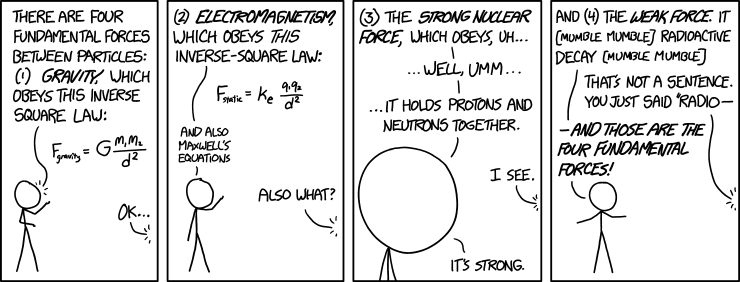
\includegraphics[scale=0.5]{fundamental_forces}

\begin{quote}
  \begin{itemize}
  \item[--]  Of these four forces, there's one we don't really understand.
  \item[--] Is it the weak force or the strong?
  \item[--]It's gravity.
  \end{itemize}
\end{quote}
\url{http://xkcd.com/1489/}

\section{Contenido de partículas}

\begin{frame}[fragile,allowframebreaks]
La materia conocida esta constituida de un cojunto de \emph{fermiones de Dirac} elementales definidos en la Tabla~\ref{tab:ef}
\begin{table}
  \centering
  \begin{tabular}{l|l|c|r}
    Tipo &Nombre & Simbolo&Carga\\\hline{}
   leptones& electrón & $e$& $-1$\\
          & neutrino & $\nu$ & $0$\\\hline{}
   quarks &quark up  & $u_1,u_2,u_3$ & $2/3$\\
          &quark down  & $d_1,d_2,d_3$& $-1/3$\\
  \end{tabular}
  \caption{Fermiones elementales:  The symbol represent both the particle, e.g $e^-$, as the antiparticle, e.g, $e^+$. The lectric chage is given in units of the electron chage $e$  }
  \label{tab:ef}
\end{table}
donde podemos definir los tripletes de color de quarks como
\begin{align}
  u=&
  \begin{pmatrix}
    u_1 \\ u_2\\ u_3\\
  \end{pmatrix}
  &d=&
  \begin{pmatrix}
    d_1 \\ d_2 \\ d_3\\
  \end{pmatrix}
\end{align}

Este conjunto de partículas esta bien definido para interacciones que conservan paridad como la interacción electromagnética o la fuerte. Para introducir la interacciones débiles usaremos más bien espinores de Weyl

\end{frame}

\section{Interacciones débiles}
\begin{frame}[fragile,allowframebreaks]
Las interacciones débiles son las responsables, entre otros fenoménos,
del decaimiento de neutrones libres en un protón, un electron y un
anti-neutrino electrónico. En nuestro entendimiento actual, se asume
que dicho decaimiento esta medidado por un bosón vectorial masivo y
cargado llamado $W^-_{\mu}$ con su correspondiente antipartícula
$W^{+}_{\mu}$. El caracter másivo da cuenta del corto alcance de la
interacción comparado con el rango infinito de la
interacción electromagnética mediada por un fotón sin masa
$A_{\mu}$. En la primera parte del decaimiento, el neutrón decae al
proton y un $W^{-}_{\mu}$ virtual, el cual a su vez decae en un
anti-neutrino derecho y un electrón izquierdo como se muestra en la
figura~\ref{fig:wnl}.

\begin{figure}
  \centering
  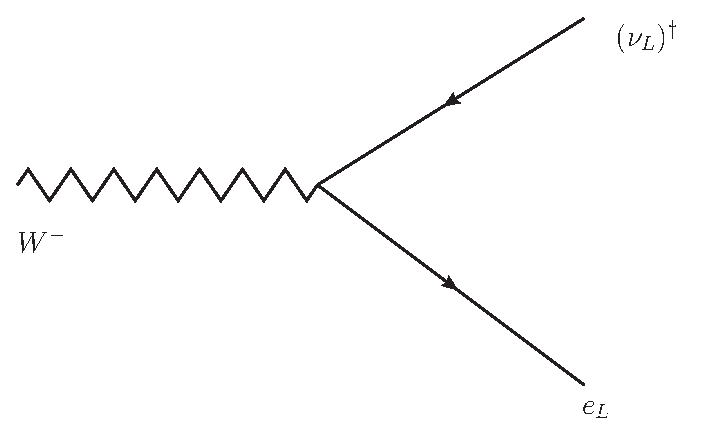
\includegraphics[scale=0.5]{wnl}
  \caption{Decaimiento del $W_\mu^-$.}
  \label{fig:wnl}
\end{figure}

Dicho decaimiento debe involucrar un término de interacción del tipo
\begin{align}
  \mathcal{L}_{W}\propto \left( \nu_L \right)^{\dagger}\overline{\sigma}^{\mu} e_L W_{\mu}^{+}.
\end{align}



Este tipo de interacción significa que en el contexto de las interacciones débiles un $e_L$ debe ser completamente
equivalente a un campo $\nu_L$. Es decir, el Lagrangiano debe ser
invariante bajo una transformación $SU(2)_L$ de esos campos. A las energías normales, a las que se encuentra por ejemplo un neutrón dentro de un núcleo de Uranio, dicha simetría permanece oculta pues un electrón izquierdo y un neutrino izquierdo son campos completamente diferentes.
La
diferencia entre ellos está en sus respectivas cargas electricas y sus
masas, pues la masa del neutrino es mucho más pequeña que la del electrón. 

Para poder explicar dicha interacción en el contexto de una simetría gauge local $SU(2)_L$, debemos asumir que dicha simetría es explicita en alguna otra escala de energía donde en efecto  $e_L$ sea completamente
equivalente a $\nu_L$.

Debemos asumir entonces que ambos campos tienen una misma hipercarga,
asociada a una nueva simetría Abeliana $\operatorname{U}(1)_Y$ que sea la precursora de la simetría Abeliana de carga eléctrica $\operatorname{U}(1)_Q$. En tal caso, podríamos esperar que
la corriente electromagnética apropiada pueda obtenerse a partir del
Grupo semisimple $SU(2)_L\times U(1)_Y$. Además. la respectiva masa para $W_{\mu}^{-}$
se podría obtener a partir del mecanismo de Higgs.

La simetría $SU(2)_L$ entre las partes izquierdas del neutrino y el electrón, y entre las partes izquierdas de los quarks up y down, se establece  definiendo los dobletes:
  \begin{align}
    L\equiv\begin{pmatrix}
      \nu_L\\
      e_L      
    \end{pmatrix}\qquad   Q=&\begin{pmatrix}
    u_L\\
    d_L
  \end{pmatrix}\,,
  \end{align}
De otro lado, La invarianza bajo $U(1)_Y$ requiere que
\begin{align}
  Y_L=&Y_{\nu_L}=Y_{e_L}\nonumber\\
  Y_Q=&Y_{u_L}=Y_{d_L}\,.
\end{align}
El generador de carga eléctrica $\widehat{Q}$, se va obtener a partir de una combinación lineal del generador diagonal de $SU(2)_L$, $T_3$, y del generador de hipercarga, $\widehat{Y}$.

Para considerar las interacciones débiles en conjunto con las interacciones electromágneticas y fuertes, es conveniente definir los campos de la primera generación en términos de los espinores ($\xi_{\alpha}$) y anti-espinores ($\eta^{\alpha}$) de Weyl izquierdos, de acuerdo a las convenciones de la Tabla~\ref{tab:electron}. El contenido de partículas con sus propiedades de transformación bajo el Grupo semisimple $SU(3)_c\times SU(2)_L\times U(1)_Y$ está dado en la Tabla~\ref{tab:fgw}
\begin{table}
  \centering
  \begin{tabular}{l|c|c}\hline
    Nombre & Símbolo & $\left( SU(3)_c, SU(2)_L, U(1)_Y \right)$\\\hline
    $\Xi_{1\alpha}$: Doblete leptónico & $L=\displaystyle{\begin{pmatrix}
      \nu_L\\
      e_L      
    \end{pmatrix}}$ & $\left( \mathbf{1},\mathbf{2},Y_L \right)$\\
    $\Xi_{2\alpha}$: Doblete de quarks & $Q=\displaystyle{\begin{pmatrix}
      u_L\\
      d_L      
    \end{pmatrix}}$ & $\left( \mathbf{3},\mathbf{2},Y_Q \right)$\\
   $\eta^{\alpha}_1$: positrón izquierdo & $\left( e_R \right)^{\dagger}$&$\left(\mathbf{1},\mathbf{1},Y_{E}\right)$ \\
   $\eta^{\alpha}_2$: anti-up izquierdo & $\left( u_R \right)^{\dagger}$&$\left(\overline{\mathbf{3}},\mathbf{1},Y_{U}\right)$ \\
   $\eta^{\alpha}_3$: anti-down izquierdo & $\left( d_R \right)^{\dagger}$&$\left(\overline{\mathbf{3}},\mathbf{1},Y_{D}\right)$ \\
  \end{tabular}
  \caption{Spinores de Weyl izquierdos para la primera generación del modelo estándar}
  \label{tab:fgw}
\end{table}

Donde el $\mathbf{3}$ o el $\overline{\mathbf{3}}$ de $SU(3)_c$ quieren decir que, además, para cada quark
\begin{align}
u_L=&
\begin{pmatrix}
  {u_{L}}_1\\
  {u_{L}}_2\\
  {u_{L}}_3
\end{pmatrix}&
  \left( u_R \right)^{\dagger}=&
  \begin{pmatrix}
    \left( u_R \right)^{\dagger}_1&
        \left( u_R \right)^{\dagger}_2&    \left( u_R \right)^{\dagger}_3
  \end{pmatrix},
\end{align}
etc.

Bajo la simetría $SU(2)_L$, los campos transforman como:
 \begin{align}
  L\to L'=&\exp(i T^i \theta_i)L\approx(1+i T^i\theta_i)L\nonumber\\
  Q\to Q'=&\exp(i T^i \theta_i)Q\approx(1+i T^i\theta_i)Q\nonumber\\
  e_R\to& e'_R=e_R\nonumber\\
  u_R\to& u'_R=u_R\nonumber\\
  d_R\to& d'_R=d_R\,.
\end{align}
donde
\begin{align}
  T^i=\frac{\tau^i}{2}\,,
\end{align}
y $\tau^i$ son las matrices de Pauli dadas en la ec.~\eqref{eq:paulimatr}.

\end{frame}



\section{Simetría gauge local $SU(3)_c\times  SU(2)_L\times  U(1)_Y$}
\begin{frame}[fragile,allowframebreaks]
Los términos de masa de Dirac, usando las convenciones de la
Tabla~\ref{tab:fgw} no son invariantes bajo la simetría $SU(2)_L$ porque
no hay forma de escribir términos escalares usando combinaciones los
campos $\Xi$ y $\eta$.  De la ec.~\eqref{eq:dwlag}, y usando la definición para los dobletes adjuntos de $SU(2)_L$ en la ec.~\eqref{eq:Xiadj}, el Lagrangiano más
general posible para los campos de la Tabla~\ref{tab:fgw} compatibles
con las simetría de Lorentz y el grupo global $SU(3)_c\times
SU(2)_L\times U(1)_Y$ es
\begin{align}
  \mathcal{L}=&\sum_{i=1}^2i\epsilon_{ab}\widetilde{\Xi}_i^{a}\overline{\sigma}^{\mu}\partial_{\mu}\Xi_i^{b}
+\sum_{i=1}^3i\eta_{i}\sigma^{\mu}\partial_{\mu} \eta^{\dagger}_i\nonumber\\
  =&\sum_{i=1}^2i\widetilde{\Xi}_i\cdot\overline{\sigma}^{\mu}\partial_{\mu}\Xi_i
+\sum_{i=1}^3i\eta_{i}\sigma^{\mu}\partial_{\mu} \eta^{\dagger}_i\nonumber\\
=&i\widetilde{L}\cdot\overline{\sigma}^{\mu}\partial_{\mu}L+i\widetilde{Q}\cdot\overline{\sigma}^{\mu}\partial_{\mu}Q
+i(e_R)^{\dagger}\sigma^{\mu}\partial_{\mu} e_R+i(u_R)^{\dagger}\sigma^{\mu}\partial_{\mu} u_R+i
(d_R)^{\dagger}\sigma^{\mu}\partial_{\mu} d_R \nonumber\\
=&i(\nu_L)^{\dagger}\overline{\sigma}^{\mu}\partial_{\mu}\nu_L+i(e_L)^{\dagger}\overline{\sigma}^{\mu}\partial_{\mu}e_L
+i (u_L)^{\dagger}\overline{\sigma}^{\mu}\partial_{\mu}u_L+i(d_L)^{\dagger}\overline{\sigma}^{\mu}\partial_{\mu}d_L \nonumber\\
&+i(e_R)^{\dagger}\sigma^{\mu}\partial_{\mu}e_R+i(u_R)^{\dagger}\sigma^{\mu}\partial_{\mu} u_R+i(d_R)^{\dagger}\sigma^{\mu}\partial_{\mu} d_R \,,
\end{align}
donde
\begin{align}
\label{eq:widetildeLQ}
  \widetilde{L}=&
  \begin{pmatrix}
   \left(e_L\right)^{\dagger}\\
  - \left(\nu_L  \right)^{\dagger}\\
  \end{pmatrix},&
  \widetilde{Q}=&
  \begin{pmatrix}
   \left(d_L\right)^{\dagger}\\
  - \left(u_L  \right)^{\dagger}\\
  \end{pmatrix},&
\end{align}
de modo que
\begin{align*}
  i\widetilde{L}\cdot\overline{\sigma}^{\mu}\partial_{\mu}L=&
  i\,\epsilon_{ab}\widetilde{L}\cdot\overline{\sigma}^{\mu}\partial_{\mu}L \nonumber\\
 =&i\,\widetilde{L}^1\overline{\sigma}^{\mu}\partial_{\mu}L^2-i\,\left( -\widetilde{L}^2 \right)\overline{\sigma}^{\mu}\partial_{\mu}L^1    \nonumber\\
 =&i\,\left( e_L \right)^{\dagger}\overline{\sigma}^{\mu}\partial_{\mu}e_L+i\,\left( \nu_L \right)^{\dagger}\overline{\sigma}^{\mu}\partial_{\mu}\nu_L    \nonumber\\
\end{align*}
y lo mismo para $Q$.



Para obtener la interacciones del modelo estándar, reemplazamos las derivadas normales por derivadas covariantes.

Proponemos entonces el Lagrangiano
\begin{align}
\label{eq:L0}
     \mathcal{L}=&i\widetilde{Q}\cdot \overline{\sigma}^\mu\mathcal{D}_\mu Q+i\widetilde{L}\cdot \overline{\sigma}^\mu\mathcal{D}_\mu L+
i(e_R)^{\dagger}\sigma^\mu\mathcal{D}_\mu {e_R}+i(d_R)^{\dagger}\sigma^\mu\mathcal{D}_\mu d_R+i(u_R)^{\dagger}\sigma^\mu\mathcal{D}_\mu {u_R}
\nonumber\\
     &-\tfrac{1}{4}G^{\mu\nu}_a G_{\mu\nu}^a-\tfrac{1}{4}W^{\mu\nu}_i W_{\mu\nu}^i-\tfrac{1}{4}B^{\mu\nu} B_{\mu\nu}\,,
\end{align}
donde
\begin{align}
  \mathcal{D}^\mu&\equiv\partial^\mu-i g_s\frac{\lambda^a}{2}G^\mu_a-i g \frac{\tau^i}{2}W^\mu_i-i {g_1}YB^\mu\,.
\end{align}
y además
\begin{align*}
  \Lambda^a\equiv\frac{\lambda^a}{2},\ a=1,2,\ldots,8 &\qquad\text{8 generadores de $SU(3)_c$}\\
  T^i\equiv\frac{\tau^i}{2},\ i=1,2,3 &\qquad\text{3 generadores de $SU(2)_L$}\\
  Y &\qquad\text{generador de $U(1)_Y$},
\end{align*}
A este nivel, tanto los 15 fermiones de Weyl (cada quark iquierdo y derecho viene en tres colores), como los 12 bosones gauge, \emph{tienen masa nula}. Necesitamos entonces un mecanismo de ruptura espontánea de simetría para generar por lo menos masa para los tres bosones gauge asociados a la interacción débil, el cual será abordado en la Sección~\ref{sec:rupt-espont-de}.



\end{frame}
Además,
\begin{align}
  W_{\mu \nu}^i=&\partial_\mu W_\nu^i -\partial_\mu W_\mu^i+ g \epsilon_{ijk}W_\mu^j W_\nu^k \nonumber\\
  B_{\mu \nu}=&\partial_\mu B_\nu -\partial_\mu B_\mu\,.
\end{align}
y $G_{\mu\nu}^a$ en ec.~\eqref{eq:258qft}.

Bajo una transformación gauge local las derivadas covariantes de los campos (y por consiguiente los campos) transforman como:
\begin{align}
  \mathcal{D}_\mu L&\to\left(\mathcal{D}_\mu L\right)'=\exp\left(-i\theta_iT^i-i\beta Y_L\right)\mathcal{D}_\mu L\nonumber\\
  \mathcal{D}_\mu Q&\to\left(\mathcal{D}_\mu Q\right)'=\exp\left(-i\alpha_a\Lambda^a-i\theta_iT^i-i\beta Y_Q\right)\mathcal{D}_\mu Q\nonumber\\
  \mathcal{D}_\mu \Phi&\to\left(\mathcal{D}_\mu \Phi\right)'=\exp\left(-i\theta_iT^i-i\beta Y_\Phi\right)\mathcal{D}_\mu \Phi\nonumber\\
  \mathcal{D}_\mu e_R&\to\left(\mathcal{D}_\mu e_R\right)'=\exp\left(-i\beta Y_{E}\right)\mathcal{D}_\mu e_R=\exp\left(-i\beta Q_{e}\right)\mathcal{D}_\mu e_R\nonumber\\
  \mathcal{D}_\mu d_R&\to\left(\mathcal{D}_\mu d_R\right)'=\exp\left(-i\alpha_a\Lambda^a-i\beta Y_{D}\right)\mathcal{D}_\mu d_R=\exp\left(-i\alpha_a\Lambda^a-i\beta Q_{d}\right)\mathcal{D}_\mu d_R\nonumber\\
  \mathcal{D}_\mu u_R&\to\left(\mathcal{D}_\mu u_R\right)'=\exp\left(-i\alpha_a\Lambda^a-i\beta Y_{U}\right)\mathcal{D}_\mu u_R=\exp\left(-i\alpha_a\Lambda^a-i\beta Q_{u}\right)\mathcal{D}_\mu u_R\,.
\end{align}
donde $Q_{e}=-1$, etc, son las cargas eléctricas asociadas a los campos.


\section{Ruptura espontánea de simetría}
\label{sec:rupt-espont-de}

\begin{frame}[fragile,allowframebreaks]
Todas las partículas en este lagrangiano son no masivas. Esto funciona sólo para los gluones y uno de los bosones gauge abelianos, pero no es realista para los bosones gauge cargados. 
Para solucionar este problema se postula la existencia de un nuevo doblete escalar complejo
( y su correspondiente adjunto de $SU(2)$) con cuatro grados de libertad:
\begin{align}
\label{eq:Phi}
  \Phi=&
  \begin{pmatrix}
    \phi^+\\
    \phi^0\\
  \end{pmatrix}=
  \begin{pmatrix}
    \phi_1+i\phi_2\\
\phi_3+i\phi_4
  \end{pmatrix},&
\widetilde{\Phi}=&
  \begin{pmatrix}
    \left( \phi^0 \right)^{*}\\
   -\phi^-\\
  \end{pmatrix}\,.
\end{align}
El  ``$\pm$'' y el superíndice 0, se ponen de forma conveniente para obtener expresiones consitentes. Es claro que $\left( \phi^+ \right)^{*}=\phi^-\,.$





Es posible ahora construir invariantes $SU(2)$ con las siguientes combinaciones de campos similares al del término de masa de Dirac en~\eqref{eq:dwlag}
\begin{align}
 -\eta_1\,\Xi_1^{a}\cdot\widetilde{\Phi}-\left(\eta_1\,\Xi_1^{a}\cdot\widetilde{\Phi}  \right)^{\dagger}
 =& -\eta_1\,\Xi_1^{a}\cdot\widetilde{\Phi}-\text{h.c}\nonumber\\
 =& -\eta^{b}_1\,\epsilon_{ab}\,\Xi_1^{a}\cdot\widetilde{\Phi}^{b}-\text{h.c} \nonumber\\
   =&-\left( e_R \right)^{\dagger}\epsilon_{ab}L^a\widetilde{\Phi}^b -\text{h.c} \nonumber\\
   =&\left( e_R \right)^{\dagger}L^1\widetilde{\Phi}^2+\left( e_R \right)^{\dagger}L^1\widetilde{\Phi}^2 +\text{h.c} \nonumber\\
   =&\left( e_R^{-} \right)^{\dagger}\nu_L\phi^- +\left( e_R^{-} \right)^{\dagger}e_L^-\phi^0 +\text{h.c} \,,
 \end{align}
donde $\text{h.c}$, denota el hermítico conjugado de cada término (para garantizar que el Lagrangiano sea real)
y hemos puesto la carga del electrón para hacer explícita la conservación de la carga eléctrica. 

Note que
\begin{align}
  \left( e_R \right)^{\dagger}\epsilon_{ab}L^a\widetilde{\Phi}^b=\left( e_R \right)^{\dagger}L\cdot \widetilde{\Phi}\,.
\end{align}


\end{frame}
\begin{frame}[fragile,allowframebreaks]
El Lagrangiano completo involucrando estos campos es
\begin{align}
     \mathcal{L}=&i\widetilde{Q}\cdot \overline{\sigma}^\mu\mathcal{D}_\mu Q+i\widetilde{L}\cdot \overline{\sigma}^\mu\mathcal{D}_\mu L+
i(e_R)^{\dagger}\sigma^\mu\mathcal{D}_\mu {e_R}+i(d_R)^{\dagger}\sigma^\mu\mathcal{D}_\mu {d_R}+i(u_R)^{\dagger}\sigma^\mu\mathcal{D}_\mu {u_R}
\nonumber\\
     &-\tfrac{1}{4}G^{\mu\nu}_a G_{\mu\nu}^a-\tfrac{1}{4}W^{\mu\nu}_i W_{\mu\nu}^i-\tfrac{1}{4}B^{\mu\nu} B_{\mu\nu}\nonumber\\
     &+\widetilde{\left( \mathcal{D}_\mu{\Phi} \right)}\cdot\mathcal{D}^\mu\Phi-\mu^2\widetilde{\Phi}\cdot\Phi-\lambda \left( \widetilde{\Phi}\cdot\Phi \right)^2\nonumber\\
     &- \left[  h_e \left( e_R \right)^{\dagger}\,L\cdot \widetilde{\Phi}_b +
      h_d \left( d_R \right)^{\dagger}\,Q\cdot \widetilde{\Phi} +
      h_u \left( u_R \right)^{\dagger}\,Q\cdot {\Phi}+\text{h.c}\right]\nonumber\\
     =&\mathcal{L}_{\text{fermion}}+\mathcal{L}_{\text{gauge}}
     +\mathcal{L}_{WBH}
     -\mathcal{L}_{\text{Yukawa}}\,.
\end{align}
donde $\mu^2<0$, y $\lambda>0$,
\begin{align}
  \widetilde{\Phi}=&i\tau_2\Phi^* 
% \nonumber\\
% =&i
% \begin{pmatrix}
%   0 & -i \\
%  i & 0\\
% \end{pmatrix}
% \begin{pmatrix}
%   \phi^+\\
% \phi^0
% \end{pmatrix}^{*} \nonumber\\
% =&\begin{pmatrix}
%   0 & 1 \\
%  -1 & 0\\
% \end{pmatrix}
% \begin{pmatrix}
%   \phi^-\\
% {\phi^0}^{*}
%\end{pmatrix} \nonumber\\
=\begin{pmatrix}
{\phi^0}^{*}\\
-  \phi^-\\
\end{pmatrix}, &   \Phi=&
  \begin{pmatrix}
    \phi^+\\
    \phi^0\\
  \end{pmatrix}.
\end{align}

\end{frame}
\begin{frame}[fragile,allowframebreaks]
Resumiendo

\begin{align}
  \label{eq:smscalar}
\mathcal{L}_{\text{fermion}}=&i\widetilde{Q}\cdot \overline{\sigma}^\mu\mathcal{D}_\mu Q+i\widetilde{L}\cdot \overline{\sigma}^\mu\mathcal{D}_\mu L \nonumber\\
&+i(e_R)^{\dagger}\sigma^\mu\mathcal{D}_\mu {e_R}+i(d_R)^{\dagger}\sigma^\mu\mathcal{D}_\mu {d_R}+i(u_R)^{\dagger}\sigma^\mu\mathcal{D}_\mu {u_R}\nonumber\\
  \mathcal{L}_{WBH}=&\widetilde{\left( \mathcal{D}_\mu{\Phi} \right)}\cdot\mathcal{D}^\mu\Phi-\mu^2\widetilde{\Phi}\cdot\Phi-\lambda \left( \widetilde{\Phi}\cdot\Phi \right)^2 \nonumber\\
\mathcal{L}_{\text{gauge}}=& -\tfrac{1}{4}G^{\mu\nu}_a G_{\mu\nu}^a-\tfrac{1}{4}W^{\mu\nu}_i W_{\mu\nu}^i-\tfrac{1}{4}B^{\mu\nu} B_{\mu\nu}\nonumber\\
  % =&(\mathcal{D}_\mu\Phi)^\dagger\mathcal{D}^\mu\Phi-\mu^2\Phi^\dagger\Phi-\lambda(\Phi^\dagger\Phi)^2\nonumber\\
%=&(\mathcal{D}_\mu\widetilde{\Phi})^\dagger\mathcal{D}^\mu\widetilde{\Phi}-\mu^2\widetilde{\Phi}^\dagger\widetilde{\Phi}-\lambda(\widetilde{\Phi}^\dagger\widetilde{\Phi})^2\nonumber\\
-\mathcal{L}_{\text{Yukawa}}=&  h_e \left( e_R \right)^{\dagger}\,L\cdot \widetilde{\Phi}_b +
      h_d \left( d_R \right)^{\dagger}\,Q\cdot \widetilde{\Phi} +
      h_u \left( u_R \right)^{\dagger}\,Q\cdot {\Phi}+\text{h.c}
\end{align}
Para el potencial escalar usaremos la forma más conveniente del producto matricial para el invariante de $SU(2)_L$ por que no hay ambiguedad con el conjugado de un campo escalar.


El potencial escalar contiene los términos
\begin{align}
  V(\Phi)=\mu^2\widetilde{\Phi}\cdot\Phi+\lambda \left( \widetilde{\Phi}\cdot\Phi \right)^2 
\end{align}
con $\mu^2<0$ y $\lambda>0$. % se reduce a
% \begin{align}
%   V(H)=\frac{1}{2}\mu^2(H+v)^2+\frac{1}{4}\lambda (H+v)^4\,.
% \end{align}


El modelo estándar es entonces una combinación de una teoría gauge local $\operatorname{SU}(3)_{c}$ con una simetría gauge local con ruptura espontánea de simetría (RES) $\operatorname{SU}(2)_L\times \operatorname{U}(1)_Y$. A continuación nos enfocaremos de momento en la parte leptónica de  $\operatorname{SU}(2)_L\times \operatorname{U}(1)_Y$ con RES.

\section{Una teoría para leptones}
Comenzaremos analizando el de sólo leptones de la primera de la primera generación, 
\begin{align}
  \label{eq:smscalarlep}
\mathcal{L}_{\text{fermion}}^{\text{lepton}}=&i\widetilde{L}\cdot \overline{\sigma}^\mu\mathcal{D}_\mu L 
+i(e_R)^{\dagger}\sigma^\mu\mathcal{D}_\mu {e_R}\nonumber\\
  \mathcal{L}_{WBH}=&\widetilde{\left( \mathcal{D}_\mu{\Phi} \right)}\cdot\mathcal{D}^\mu\Phi-\mu^2\widetilde{\Phi}\cdot\Phi-\lambda \left( \widetilde{\Phi}\cdot\Phi \right)^2 \nonumber\\
\mathcal{L}_{\text{gauge}}=& -\tfrac{1}{4}G^{\mu\nu}_a G_{\mu\nu}^a-\tfrac{1}{4}W^{\mu\nu}_i W_{\mu\nu}^i-\tfrac{1}{4}B^{\mu\nu} B_{\mu\nu}\nonumber\\
  % =&(\mathcal{D}_\mu\Phi)^\dagger\mathcal{D}^\mu\Phi-\mu^2\Phi^\dagger\Phi-\lambda(\Phi^\dagger\Phi)^2\nonumber\\
%=&(\mathcal{D}_\mu\widetilde{\Phi})^\dagger\mathcal{D}^\mu\widetilde{\Phi}-\mu^2\widetilde{\Phi}^\dagger\widetilde{\Phi}-\lambda(\widetilde{\Phi}^\dagger\widetilde{\Phi})^2\nonumber\\
-\mathcal{L}_{\text{Yukawa}}^{\text{lepton}}=&  h_e \left( e_R \right)^{\dagger}\,L\cdot \widetilde{\Phi}_b +\text{h.c}
\end{align}
sin perdida de generalidad para $\mathcal{L}_{\text{gauge}}$ y $ \mathcal{L}_{WBH}\,$.

\subsection{Interacciónes débiles fermión-gauge para leptones}

Nos enfocaremos de momento en la parte leptónica pues las interacciones para quarks involucran el mismo tipo de cálculos.

Los términos de interacción generados por la simetría gauge para el sector leptónico son:
\begin{align}
\label{eq:devLW}
 \mathcal{L}_{\text{fermion}}^{\text{lepton}}=& i \widetilde{L}\cdot\overline{\sigma}^\mu\mathcal{D}_\mu L+  i \left( e_R \right)^{\dagger}{\sigma}^\mu\mathcal{D}_\mu e_R \nonumber\\
=&i \widetilde{L}\cdot\overline{\sigma}^\mu\partial_\mu L+i \left(e_R  \right)^{\dagger}\sigma^\mu\partial_\mu {e_R} \nonumber\\
&+ i \widetilde{L}\cdot\overline{\sigma}^\mu(-i g_2 T_iW_\mu^i-i {g_1}\,Y_LB_\mu) L + i \left( e_R \right)^{\dagger}\sigma^\mu \left( -i{g_1} Y_E B_{\mu} \right) {e_R}\,.
\end{align}
Definiendo
\begin{align}
\label{eq:knt}
  \mathcal{L}_{\text{kinetic}}=&i \widetilde{L}\cdot\overline{\sigma}^\mu\partial_\mu L+i \left(e_R  \right)^{\dagger}\sigma^\mu\partial_\mu {e_R} \\
  \mathcal{L}_{WBL}=&i \widetilde{L}\cdot\overline{\sigma}^\mu(-i g_2 T_iW_\mu^i-i {g_1}\,Y_LB_\mu) L + i \left( e_R \right)^{\dagger}\sigma^\mu \left( -i{g_1} Y_E B_{\mu} \right) {e_R}\nonumber\,.
\end{align}
tenemos que
\begin{align}
\mathcal{L}_{WBL}=& \widetilde{L}\cdot\overline{\sigma}^\mu(g_2 T_1W_\mu^1+ g_2 T_2W_\mu^2+g_2 T_3W_\mu^3+{g_1}\,Y_LB_\mu) L+ g_1 Y_E\left(e_R \right)^{\dagger}\sigma^\mu  {e_R} B_\mu\nonumber\\
=& \widetilde{L}\cdot\overline{\sigma}^\mu\left[\frac{g_2}{\sqrt{2}}
  \begin{pmatrix}
0 & W_\mu^+\\
W_\mu^- & 0\\    
  \end{pmatrix}
+g_2 T_3W_\mu^3+{g_1}\,Y_LB_\mu
\right]L+ {g_1} Y_E\left(e_R \right)^{\dagger}\sigma^\mu  {e_R} B_\mu\nonumber\\
=&i \widetilde{L}\cdot\overline{\sigma}^\mu\frac{g_2}{\sqrt{2}}
  \begin{pmatrix}
0 & W_\mu^+\\
W_\mu^- & 0\\    
  \end{pmatrix}L+
 \widetilde{L}\cdot\overline{\sigma}^\mu\left[g_2 T_3W_\mu^3+{g_1}\,Y_LB_\mu
\right]L+ {g_1} Y_E\left(e_R \right)^{\dagger}\sigma^\mu  {e_R} B_\mu\nonumber\\
  =& \frac{g_2}{\sqrt{2}}\widetilde{L}\cdot\overline{\sigma}^\mu
  \begin{pmatrix}
e_LW_\mu^+\\
\nu_L W_\mu^-\\    
  \end{pmatrix}+\mathcal{L}_{A Z L}\,,
\end{align}

donde
\begin{align}
\label{eq:lazl}
  \mathcal{L}_{A Z L}=& \widetilde{L}\cdot\overline{\sigma}^\mu\left[g_2 T_3W_\mu^3+{g_1}\,Y_LB_\mu\right]L+ {g_1} Y_E\left(e_R \right)^{\dagger}\sigma^\mu  {e_R} B_\mu\,.
\end{align}

Teniendo en cuenta que 
\begin{align}
  \frac{g_2}{\sqrt{2}}\widetilde{L}\cdot\overline{\sigma}^\mu
  \begin{pmatrix}
e_LW_\mu^+\\
\nu_L W_\mu^-\\    
  \end{pmatrix}=\frac{g_2}{\sqrt{2}} \left[ \epsilon^{12} \widetilde{L}_1 \overline{\sigma}^{\mu} \nu_L W_{\mu}^-
+\epsilon^{21}  \widetilde{L}_2 \overline{\sigma}^{\mu} e_L W_{\mu}^+ \right],
\end{align}
y usando \eqref{eq:widetildeLQ}
\begin{align}
  \frac{g_2}{\sqrt{2}}\widetilde{L}\cdot\overline{\sigma}^\mu
  \begin{pmatrix}
e_LW_\mu^+\\
\nu_L W_\mu^-\\    
  \end{pmatrix}=\frac{g_2}{\sqrt{2}} \left[\left( e_L \right)^{\dagger} \overline{\sigma}^{\mu} \nu_L W_{\mu}^-
+ \left( \nu_L \right)^{\dagger} \overline{\sigma}^{\mu} e_L W_{\mu}^+ \right].
\end{align}
De este modo, la simetría gauge genera la interacción deseada con los bosones gauge cargados $W_{\mu}^{\pm}$. Sin embargo, se generan muchas otras interacciones las cuales deben contener apropiadamente la interacción electromagnética en algún cambio de base.

% Reemplazando en \eqref{eq:devLW}
% \begin{align}
%     i \widetilde{L}\cdot\overline{\sigma}^\mu\mathcal{D}_\mu L-i \widetilde{L}\cdot\overline{\sigma}^\mu\partial_\mu L
%   =&
% \frac{g_2}{\sqrt{2}}\left[\left( \nu_L \right)^{\dagger}\overline{\sigma}^\mu e_LW_\mu^++
% \left( e_L \right)^{\dagger}\overline{\sigma}^\mu\nu_L W_\mu^-\right]    
% +\mathcal{L}_{A Z L}\nonumber\\
%   =&
% \mathcal{L}_{W L}    
% +\mathcal{L}_{A Z L}\,,
% \end{align}
Entonces
\begin{align}
  \mathcal{L}_{WBL}= \mathcal{L}_{W L}+  \mathcal{L}_{A Z L}\,,
\end{align}
donde
\begin{align}
\label{eq:lwl}
  \mathcal{L}_{W L}=&\frac{g_2}{\sqrt{2}}\left[\left( \nu_L \right)^{\dagger}\overline{\sigma}^\mu e_LW_\mu^++
\left( e_L \right)^{\dagger}\overline{\sigma}^\mu\nu_L W_\mu^-\right].
\end{align}

El prinicipal problema con $\mathcal{L}_{AZL}$ en la ec.~\eqref{eq:lazl} es que el neutrino izquierdo $\nu_L$ presente en $L$ se acopla a los dos bosones gauge neutros $W_3^{\mu}$ y $B^{\mu}$. Debemos buscar una base en la cual recuperar la interacción electromagnética en la cual el fotón $A_{\mu}$ no se acopla a partículas neutras como el $\nu_L$. Definimos entonces el posible fotón a partir de la rotación
\begin{equation}
\label{eq:rottw}
  \begin{pmatrix}
    W^3_\mu\\
    B_\mu
  \end{pmatrix}=\begin{pmatrix}
    \cos\theta_W & \sin\theta_W\\
    -\sin\theta_W& \cos\theta_W
  \end{pmatrix}
  \begin{pmatrix}
    Z_\mu\\
    A_\mu
  \end{pmatrix}.
\end{equation}
Aplicando esta rotación a~\eqref{eq:lazl}, tenemos que
\begin{align}
\label{eq:brot}
   \mathcal{L}_{A Z L}=& \widetilde{L}\cdot\overline{\sigma}^\mu\left[g_2 T_3(c_W Z_\mu+s_W A_\mu)+{g_1}\,Y_L(-s_W Z_\mu+c_W A_\mu)\right]L
    +g_1 Y_E\left(e_R \right)^{\dagger}\sigma^\mu  {e_R} (-s_W Z_\mu+c_W A_\mu)\nonumber\\
     =& \widetilde{L}\cdot\overline{\sigma}^\mu\left[g_2 T_3c_W Z_\mu+g_2 T_3s_W A_\mu-{g_1}\,Y_Ls_W Z_\mu+{g_1}\,Y_Lc_W A_\mu\right]L\nonumber\\
&-g_1 s_W Y_E\left(e_R \right)^{\dagger}\sigma^\mu  {e_R}Z_{\mu}  +g_1 c_W Y_E\left(e_R \right)^{\dagger}\sigma^\mu  {e_R}A_{\mu}  \nonumber\\
    =& \widetilde{L}\cdot\overline{\sigma}^\mu\left[\left(g_2 c_WT_3-{g_1}s_W\,Y_L\right)Z_\mu
       +\left(g_2 s_W T_3+{g_1}c_W\,Y_L\right) A_\mu\right]L \nonumber\\
&-g_1 s_W Y_E\left(e_R \right)^{\dagger}\sigma^\mu  {e_R}Z_{\mu}  +g_1 c_W Y_E\left(e_R \right)^{\dagger}\sigma^\mu  {e_R}A_{\mu}  \,,
\end{align}
donde $c_W=\cos\theta_W$, $s_W=\sin\theta_W$. 

Para identificar $A_{\mu}$ con el fotón, debemos imponer la condición
\begin{align}
e\widehat{Q}=g_2 s_W T_3+{g_1}c_W\,\widehat{Y}\,.
\end{align}
De este modo
\begin{align}
  e\widehat{Q}L =& \left(g_2 s_W T_3+{g_1}c_W\,\widehat{Y}\right) L \nonumber\\
=& \left(g_2 s_W T_3+{g_1}c_W\,Y_L\right) L \,,
\end{align}
y
\begin{align}
 e\widehat{Q} e_R =& \left(g_2 s_W T_3+{g_1}c_W\,\widehat{Y}\right) e_R\nonumber\\  
=& g_1 c_W\,Y_E \, e_R\,.
\end{align}
Separando las condiciones sobre los coeficientes de las condiciones sobre los generadores, tenemos las dos condiciones equivalentes
\begin{align}
\label{eq:esc}
    e=&g_2\sin\theta_W=g_1 \cos\theta_W\,,
\end{align}
y
\begin{align}
\label{eq:gn}
 \widehat{Q}=&T_3+\widehat{Y}\,.
\end{align}
donde $e$ es la carga eléctrica del electrón, y $\widehat{Q}$ es el generador de carga elétrica conservada asociada a la simetría gauge local $\operatorname{U}(1)_Q$. 

La ec. \eqref{eq:gn}, se conoce como la relación de Gell-Mann--Nishijima, y junto con~\eqref{eq:esc}, establece las condiciones que se deben satisfacer para obtener apropiadamente la QED a partir de la interacción electrodébil asociada al grupo semisimple $SU(2)_L\times  U(1)_Y$.


De \eqref{eq:esc}, podemos expresar el ángulo $\theta_W$ en términos de $g_1$ y $g_2$ como
\begin{align}
\label{eq:twa}
  \tan\theta_W=\frac{g_1}{g_2}\,.
\end{align}


Usando la relación entre $g_2$ y ${g_1}$~\eqref{eq:twa} en ~\eqref{eq:brot}
\begin{align}
    \mathcal{L}_{A Z L}
=&g_2 s_W \widetilde{L}\cdot\overline{\sigma}^\mu\left[\left(\cot\theta_WT_3- \tan\theta_W\,Y_L\right)Z_\mu
       +\left(T_3+Y_L\right) A_\mu\right]L \nonumber\\
&+g_2 s_W \left(e_R \right)^{\dagger}\sigma^\mu \left[ \left(0 -\tan\theta_W  Y_E  \right) Z_{\mu}  +\left( 0+ Y_E \right)  A_{\mu} \right]{e_R}\,,
\end{align}
donde hemos puesto explícitamente el cero correspondiente a: $T_3 e_R= 0 \,e_R$.

Como el generador asociado a $A_\mu$ debe ser el generador de carga eléctrica, podemos usar la primera ecuación en \eqref{eq:esc}:
\begin{align}
  e=g_2\sin\theta_W\,,
\end{align}
y si además definimos
\begin{align}
  \mathcal{L}_{E}=g_2 s_W \left(e_R \right)^{\dagger}\sigma^\mu \left[ \left(0 -\tan\theta_W  Y_E  \right) Z_{\mu}  +\left( 0+ Y_E \right)  A_{\mu} \right]{e_R}\,,
\end{align}
tenemos que
\begin{align}
\label{eq:lazlf}
    \mathcal{L}_{A Z L}
=&e \widetilde{L}\cdot\overline{\sigma}^\mu\left(\cot\theta_W T_3-\tan\theta_W\,Y_L\right)L Z_\mu
       +e \widetilde{L}\cdot\gamma^\mu \widehat{Q} L A_\mu+\mathcal{L}_E\nonumber\\
=&e \widetilde{L}\cdot\overline{\sigma}^\mu\left[\cot\theta_W T_3-\tan\theta_W\left(\widehat{Q}-T_3\right)\right]L Z_\mu
       +e \widetilde{L}\cdot\overline{\sigma}^\mu \widehat{Q} L A_\mu + \mathcal{L}_E\nonumber\\
=&\phantom{+}\frac{e}{2c_W s_W} \widetilde{L}\cdot\overline{\sigma}^\mu\left[ \tau_3-2s_W^2\widehat{Q}\right]L Z_\mu
       +e \widetilde{L}\cdot\overline{\sigma}^\mu \widehat{Q} L A_\mu \nonumber\\
&+\frac{e}{2c_W s_W} \left( e_R \right)^{\dagger}{\sigma}^\mu\left[ 0-2s_W^2\widehat{Q}\right]e_R\, Z_\mu
       +e \left( e_R \right)^{\dagger}{\sigma}^\mu \widehat{Q} e_R\, A_\mu \nonumber\\
=&\mathcal{L}_{ZL}+\mathcal{L}^{\text{int}}_{\text{QED}} \,,
\end{align}
donde
\begin{align}
     \mathcal{L}^{\text{int}}_{\text{QED}}=&e \widetilde{L}\cdot\overline{\sigma}^\mu \widehat{Q} L A_\mu+
e \left( e_R \right)^{\dagger}{\sigma}^\mu \widehat{Q} e_R\, A_\mu \nonumber\\
\mathcal{L}_{ZL}=&\frac{e}{2c_W s_W} \widetilde{L}\cdot\overline{\sigma}^\mu\left[ \tau_3-2s_W^2\widehat{Q}\right]L Z_\mu
+\frac{e}{2c_W s_W} \left( e_R \right)^{\dagger}{\sigma}^\mu\left[ 0-2s_W^2\widehat{Q}\right]e_R\, Z_\mu\,.
\end{align}


Para mostrar explícitamente que el neutrino izquierdo no se acopla al fotón y que la QED se puede recuperar, 
debemos encontrar los valores numérico para $Y_L$ y $Y_E$. Partiendo de la relación de Gell-Mann--Nishijima \eqref{eq:gn}
\begin{align}
  \widehat{Q}L=&(T_3+Y_L)L \nonumber\\
  \begin{pmatrix}
    Q_\nu & 0\\
    0  & Q_e
  \end{pmatrix}
  \begin{pmatrix}
    \nu_L\\
    e_L
  \end{pmatrix}=  
  \begin{pmatrix}
   Q_{\nu} \nu_L\\
   Q_e e_L
  \end{pmatrix}
= & \begin{pmatrix}
    \frac{1}{2} + Y_L & 0\\
    0  & -\frac{1}{2}+Y_L
  \end{pmatrix}  \begin{pmatrix}
    \nu_L\\
    e_L
  \end{pmatrix} \,,
\end{align}
podemos establecer que
\begin{align}
  Q_{\nu}&=0=\frac{1}{2}+Y_L\,, & Q_e&=-1=-\frac{1}{2}+Y_L\,,
\end{align}
lo cual  requiere que
\begin{align}
  Y_L=\frac{1}{2}\,.
\end{align}
De la misma forma
\begin{align}
  Y_E=Q_e=-1\,.
\end{align}
Note que para campos derechos la hipercarga coincide con la carga eléctrica.

Entonces
\begin{align}
     \mathcal{L}^{\text{int}}_{\text{QED}}=&e \widetilde{L}\cdot\overline{\sigma}^\mu \widehat{Q} L A_\mu+
e \left( e_R \right)^{\dagger}{\sigma}^\mu \widehat{Q} e_R\, A_\mu \nonumber\\
=&-e \left[ \left( e_L \right)^{\dagger}\overline{\sigma}^\mu \ e_L + \left( e_R \right)^{\dagger}{\sigma}^\mu \ e_R  \right]A_{\mu}\,,
\end{align}
y la interacción de la electrodinámica cuántica se recupera satisfactoriamente.

Resumiendo
\begin{align}
    i \widetilde{L}\cdot\overline{\sigma}^\mu\mathcal{D}_\mu L+  i \left( e_R \right)^{\dagger}{\sigma}^\mu\mathcal{D}_\mu e_R=&\mathcal{L}_{\text{kinetic}}+
\mathcal{L}_{WL}+ \mathcal{L}_{A Z L}\,,
\end{align}
dados en las ecs.~\eqref{eq:knt}, \eqref{eq:lwl} y \eqref{eq:lazlf}. Para obtener la interacción reqierida de los $W^{\pm}$ con el $\nu_L$ y $e_L$, el modelo gauge local $\operatorname{SU}(2)_L\times \operatorname{U}(1)_Y$ predice la existencia de nuevas interacciones con un nuevo bosón gauge $Z_{\mu}$ dadas por
\begin{align}
\mathcal{L}_{ZL}=&\mathcal{L}_{AZL}-\mathcal{L}^{\text{int}}_{\text{QED}} \nonumber\\
=&\frac{e}{2c_W s_W} \widetilde{L}\cdot\overline{\sigma}^\mu\left[ \tau_3-2s_W^2\widehat{Q}\right]L Z_\mu
+\frac{e}{2c_W s_W} \left( e_R \right)^{\dagger}{\sigma}^\mu\left[ 0-2s_W^2\widehat{Q}\right]e_R\, Z_\mu\,.
\end{align}
Una predicción bastante concreta es que los neutrinos izquierdos se acoplan con el nuevo bosón gage neutro a través del término de interacción
\begin{align}
\mathcal{L}_{Z\nu}=  \frac{e}{4c_W s_W}\left( \nu_L \right)^{\dagger} \overline{\sigma}^{\mu} \nu_L Z_\mu\,.
\end{align}
Note que a este nivel el bosón gauge $Z_{\mu}$ es no masivo. Sin embargo para explicar porque dicha interacción no había sido observada al momento de su predicción se tiene que asumir que el bosón gauge $Z_{\mu}$ debe ser muy masivo para que la interacción sea de corto alcance y por consiguiente suprimida con respecto a la de bosones gauge sin masa. 

Por lo tanto, para obtener una teoría realista se debe adicionar un mecanismo de ruptura espontánea de simetría para dar masa a los tres bosones $W_{\mu}^{+}$, $W_{\mu}^{-}$ y $Z_{\mu}$. Dicho mecanismo será discutido en la Sección~\ref{sec:el-gauge-unitario}.



\subsection{El gauge unitario}
\label{sec:el-gauge-unitario}

\begin{frame}[fragile,allowframebreaks]
Retornando al doblete de Higgs del modelo estándar en la ec.~\eqref{eq:polarhiggs}, los cuatro grados de libertad de $\Phi$, pueden escribirse en forma polar con la parte real neutra desplazada para generar la ruptura espontánea de la simetría $SU(2)_L\times  U(1)_Y$. De este modo, y sin perdida de generalidad
\begin{align}
\label{eq:92qft}
  {\Phi}=&e^{i G_j(x)T^j}
  \begin{pmatrix}
    0\\
    \frac{1}{\sqrt{2}}[H(x)+v]
  \end{pmatrix}.
\end{align}

Para $SU(2)_L\times  U(1)_Y$ tenemos cuatro generadores y cuatro bosones gauge. De acuerdo a la parametrización en ec.~\eqref{eq:92qft} esperamos que aparezcan tres bosones de Goldstone y un campo de Higgs con masa, de manera que quedará un generador no roto correspondiente a una simetría remanente del vacío $U(1)_Q$
\begin{equation}
  SU(2)_L\times  U(1)_Y\overset{\langle\widetilde{\Phi}\rangle}{\longrightarrow}U(1)_Q.
\end{equation}

Se espera entonces que el espectro consista de un bosón de Higgs, tres bosones gauge masivos, y un bosón gauge sin masa.

Podemos hacer una transformación gauge similar a la de la 
%DEBUG: corregir
ec.~\eqref{eq:93qft} sobre el campo $\widetilde{\Phi}$, tal que
\begin{equation}
  \label{eq:123qft}
    {\Phi}\to{\Phi}'=
  \begin{pmatrix}
    0\\
    \frac{1}{\sqrt{2}}(H(x)+v)
  \end{pmatrix},
\end{equation}
que define el \emph{gauge unitario}. En adelante sin embargo omitiremos las primas sobre los campos transformados ${\Phi}'$ y $W'_{\mu\nu}$.

Comenzaremos analizando la parte escalar del Lagrangiano del Modelo dada en la ec.~\eqref{eq:smscalar} en el gauge unitario
\begin{align}
  \mathcal{L}_{WBH}
  =&\widetilde{\left( \mathcal{D}_\mu{\Phi} \right)}\cdot\mathcal{D}^\mu\Phi-\mu^2\widetilde{\Phi}\cdot\Phi-\lambda \left( \widetilde{\Phi}\cdot\Phi \right)^2 \nonumber\\
  =&\frac{1}{2}\widetilde{\left[\mathcal{D}^\mu \begin{pmatrix}
    0\\
    H(x)+v
  \end{pmatrix}\right]}\cdot \mathcal{D}_\mu\begin{pmatrix}
    0\\
    H(x)+v
  \end{pmatrix}-V(H)\,,
\end{align}
donde $V(H)$ dado en la ec.~\eqref{eq:higgspot}, incluye el término de masa para el bosón de Higgs \eqref{eq:higgsmass}:
\begin{equation}
  m_H^2=2\left|\mu^2\right|=2\lambda v^2
\end{equation}
De la ec.~\eqref{eq:w22}
\begin{align}
      W_\mu=&\begin{pmatrix}
    \frac{1}{2}W_3&\frac{1}{\sqrt{2}}W^+_\mu\\
    \frac{1}{\sqrt{2}}W^-_\mu&-\frac{1}{2}W^3_\mu
  \end{pmatrix}.
\end{align}
$\mathcal{D}_\mu$ corresponde a la matrix $2\times  2$, dada en la ec.~\eqref{eq:d22}, con el reemplazo
\begin{align}
\mp\frac{i}{2}g_2 W^3_\mu\to  -i\left(\pm\frac{1}{2}g_2 W^3_\mu+{g_1}Y B_\mu\right)
\end{align}

\begin{align}
  \label{eq:dercovsu2L}
 \mathcal{D}_\mu &=  \begin{pmatrix}
    \partial_\mu-i\left(\frac{1}{2}g_2 W^3_\mu+{\color{red}{g_1} Y B_\mu}\right)&-\frac{i}{\sqrt{2}}g_2 W^+_\mu\\
    -\frac{i}{\sqrt{2}}g_2 W^-_\mu&\partial_\mu-i\left(-\frac{1}{2}g_2 W^3_\mu+{\color{red}{g_1}Y B_\mu}\right)
  \end{pmatrix}.
\end{align}

Entonces
\begin{align}
\mathcal{D}_\mu \begin{pmatrix}
    0\\
    H(x)+v
  \end{pmatrix}=\begin{pmatrix}
    -\frac{i}{\sqrt{2}}gW_\mu^+(H+v)\\
    \partial_\mu H-i\left(-\frac{1}{2}gW^3_\mu+{\color{red}{g_1}Y_{\widetilde{\Phi}} B_\mu}\right)(H+v)
  \end{pmatrix}.
\end{align}

El correspondiente productor escalar $\operatorname{SU}(2)_L$ es:
\begin{align}
  \mathcal{L}_{WBH}=&\frac{1}{2}\widetilde{\begin{pmatrix}
    -\frac{i}{\sqrt{2}}g{W^\mu}^+(H+v)\\
    \partial^\mu H-i\left(-\frac{1}{2}gW_3^\mu+{g_1}Y_{\widetilde{\Phi}} B^\mu\right)(H+v)
  \end{pmatrix}}\cdot
   \begin{pmatrix}
    -\frac{i}{\sqrt{2}}gW_\mu^+(H+v)\\
    \partial_\mu H-i\left(-\frac{1}{2}gW^3_\mu+{g_1}Y_{\widetilde{\Phi}} B_\mu\right)(H+v)
  \end{pmatrix}-V(H)\nonumber\\
=&\frac{1}{2}\begin{pmatrix}
    \partial^\mu H+i\left(-\frac{1}{2}gW_3^\mu+{g_1}Y_{\widetilde{\Phi}} B^\mu\right)(H+v)\\
    \frac{i}{\sqrt{2}}g{W^\mu}^-(H+v)\\
  \end{pmatrix}\cdot
  \begin{pmatrix}
    -\frac{i}{\sqrt{2}}gW_\mu^+(H+v)\\
    \partial_\mu H-i\left(-\frac{1}{2}gW^3_\mu+{g_1}Y_{\widetilde{\Phi}} B_\mu\right)(H+v)
  \end{pmatrix}-V(H)\nonumber\\
  =&\frac{1}{4}g^2{W^\mu}^-W_\mu^+(H+v)^2-V(H)\nonumber\\
  &+\frac{1}{2}\left[\partial^\mu H+i\left(-\tfrac{1}{2}gW_3^\mu+{g_1}Y_{\widetilde{\Phi}} B^\mu\right)(H+v)\right]
  \times\nonumber\\
  &\qquad\left[\partial_\mu H-i\left(-\tfrac{1}{2}gW^3_\mu+{g_1}Y_{\widetilde{\Phi}} B_\mu\right)(H+v)\right]\nonumber\\
 =&-V(H)
  +\frac{1}{4}g^2{W^\mu}^-W_\mu^+(H+v)^2+\nonumber\\
  &+\frac{1}{2}\partial^\mu H\partial_\mu H+\frac{1}{2}\left(-\tfrac{1}{2}gW_3^\mu+{\color{red}{g_1}Y_{\widetilde{\Phi}} B^\mu}\right)^2(H+v)^2
\end{align}
donde la última línea corresponde a la magnitud del ``número'' complejo: 
\begin{align}
\left[\partial_\mu H-i\left(-\tfrac{1}{2}gW^3_\mu+{g_1}Y_{\widetilde{\Phi}} B_\mu\right)(H+v)\right]
\end{align}

\end{frame}
\begin{frame}[fragile,allowframebreaks]

Entonces
\begin{align}
  \label{eq:96qft}
  \mathcal{L}_{WBH}=&\frac{1}{2}\partial^\mu H\partial_\mu H-V(H)
  +\frac{g^2v^2}{4}{W^\mu}^-W_\mu^+ \left( \frac{H}{v}+1 \right)^2+\mathcal{L}_{Z A H}\,,
\end{align}
donde
\begin{align}
  \mathcal{L}_{ZAH}=\frac{1}{2}&\left(\tfrac{1}{4}g^2W_3^\mu W^3_\mu-\tfrac{1}{2}g{g_1}Y_{\widetilde{\Phi}} W_3^\mu B_\mu-\tfrac{1}{2}g{g_1}Y_{\widetilde{\Phi}} W_3^\mu B_\mu+{{g_1}}^2Y_{\widetilde{\Phi}} ^2B^\mu B_\mu\right)
\left(H+v\right)^2.
\end{align}
Haciendo $Y_{\widetilde{\Phi}} =1/2$ como en la ec.~\eqref{eq:yyy},
\begin{align}
  \mathcal{L}_{ZAH}=\frac{1}{2}\frac{v^2}{4}
  \begin{pmatrix}
    W^\mu_3 & B^\mu
  \end{pmatrix}
  \begin{pmatrix}
    g^2_2&-g_2{g_1}\\
    -g_2{g_1}&g_1^2
  \end{pmatrix}
  \begin{pmatrix}
    W^3_\mu\\
    B_\mu
  \end{pmatrix}
\left(\frac{H}{v}+1\right)^2\,.
\end{align}
Sea
\begin{equation}
  V=\begin{pmatrix}
    \cos\theta_W & \sin\theta_W\\
    -\sin\theta_W& \cos\theta_W
  \end{pmatrix}=
  \frac{1}{\sqrt{g^2_2+g_1^2}}\begin{pmatrix}
    g_2   & {g_1}\\
    -{g_1} & g_2
  \end{pmatrix},
\end{equation}
con $\tan\theta_W={g_1}/g$, tal que $g\sin\theta_W={g_1}\cos\theta_W$, como en la ec.~\eqref{eq:esc}. De esta forma podremos comprobar si la misma condición que hace que los neutrinos no se acoplen con el fotón, garantiza el campo neutro $H$ tampoco se acopla directamente con el fotón. 

Note que $V$ es una matrix ortogonal que satisface $VV^T=V^TV=\mathbf{1}$. Si (ver ec.~\eqref{eq:rottw}),
\begin{align}
  \begin{pmatrix}
    W^3_\mu\\
    B_\mu
  \end{pmatrix}=&V
  \begin{pmatrix}
    Z_\mu\\
    A_\mu
  \end{pmatrix}&\text{ó}\qquad
  \begin{pmatrix}
    Z_\mu\\
    A_\mu
  \end{pmatrix}=&V^T
  \begin{pmatrix}
    W^3_\mu\\
    B_\mu
  \end{pmatrix}
\end{align}
entonces
\begin{align}
  \mathcal{L}_{ZAH}=&\frac{1}{2}\frac{v^2}{4}
  \begin{pmatrix}
    W^{3\mu} & B^\mu
  \end{pmatrix}VV^T
  \begin{pmatrix}
    g^2&-g_2{g_1}\\
    -g_2{g_1}&g_1^2
  \end{pmatrix}VV^T
  \begin{pmatrix}
    W^3_\mu\\
    B_\mu
  \end{pmatrix}
\left(\frac{H}{v}+1\right)^2\nonumber\\
=&\frac{1}{2}\frac{v^2}{4}
  \begin{pmatrix}
    Z^\mu & A^\mu
  \end{pmatrix}\left[V^T
  \begin{pmatrix}
    g_2^2&-g_2{g_1}\\
    -g_2{g_1}&g_1^2
  \end{pmatrix}V\right]
  \begin{pmatrix}
    Z_\mu\\
    A_\mu
  \end{pmatrix}
\left(\frac{H}{v}+1\right)^2
\end{align}
\begin{align}
  V^T
  \begin{pmatrix}
    g_2^2&-g_2{g_1}\\
    -g_2{g_1}&{{g_1}}^2
  \end{pmatrix}V=&\frac{1}{g_2^2+{{g_1}}^2}
  \begin{pmatrix}
    g_2^3+g{{g_1}}^2 & -g_2^2{g_1}-{{g_1}}^3\\
+g_2^2{g_1}-g_2^2{g_1}    &-g_2 g_1^2+g_2 g_1^2
  \end{pmatrix}
\begin{pmatrix}
    g_2   & {g_1}\\
    -{g_1} & g_2
  \end{pmatrix}\nonumber\\
=&\frac{1}{g_2^2+{{g_1}}^2}
  \begin{pmatrix}
    g_2^3+g_2 g_1^2 & -g_2^2{g_1}-g_1^3\\
    0   &0
  \end{pmatrix}
\begin{pmatrix}
    g_2   & {g_1}\\
    -{g_1} & g_2
  \end{pmatrix}\nonumber\\
=&\frac{1}{g_2^2+{{g_1}}^2}
  \begin{pmatrix}
    g_2^4+g^2 g_1^2+g_2^2 g_1^2+g_1^4 & g_2^3{g_1}+g_2 g_1^3-g_2^3{g_1}-g_2 g_1^3\\
    0    &0
  \end{pmatrix}\nonumber\\
=&\begin{pmatrix}
    g_2^2+g_1^2 & 0\\
    0    &0
  \end{pmatrix}
\end{align}
De este modo

\begin{align}
  \mathcal{L}_{ZAH}&=\frac{1}{2}\frac{v^2}{4}\left(g_2^2+g_1^2\right)Z^\mu Z_\mu
  \left(\frac{H}{v}+1\right)^2\nonumber\\
 &=\frac{1}{2}\left(\frac{g_2v}{2}\right)^2\left(1+\tan^2\theta_W\right)Z^\mu Z_\mu
             \left(\frac{H}{v}+1\right)^2\nonumber\\
   &=\frac{1}{2}\left(\frac{g_2v}{2\cos\theta_W}\right)^2Z^\mu Z_\mu\left(\frac{H}{v}+1\right)^2\,.
\end{align}
Retornando a la ec.~(\ref{eq:96qft}), tenemos
tenemos
\begin{align}
  \label{eq:lwbhfin}
  \mathcal{L}_{W B H}=&\widetilde{\left( \mathcal{D}_\mu{\Phi} \right)}\cdot\mathcal{D}^\mu\Phi-\mu^2\widetilde{\Phi}\cdot\Phi-\lambda \left( \widetilde{\Phi}\cdot\Phi \right)^2 \nonumber\\
  =&\frac{1}{2}\partial^\mu H\partial_\mu H-V(H)\nonumber\\
  &+\frac{1}{2}m_W^2{W^\mu}^-W_\mu^+ \left(\frac{H}{v}+1 \right)^2
    +\frac{1}{2}m_W^2{W^\mu}^-W_\mu^+\left(\frac{H}{v}+1 \right)^2
    +\frac{1}{2}m_Z^2Z^\mu Z_\mu\left(\frac{H}{v}+1 \right)^2\,,
\end{align}
donde el termino $1$ en la expansión binomial $\left({H}/{v}+1 \right)^2$ corresponde al
término de masa en cada caso:
%instiki:
\begin{itemize} %noinstiki
\item Masas gauge:
\begin{equation}
\label{eq:mwz}
  m_W=\frac{g_2v}{2}
  \qquad 
  m_Z=\frac{g_2v}{2\cos\theta_W},
\end{equation}
y
\begin{equation}
\label{eq:mwzw}
  m_Z=\frac{m_W}{\cos\theta_W}.
\end{equation}
\item Ver eq.~\eqref{eq:higgspot}
  \begin{align}
    V(H)=&\tfrac{1}{2}m_H^2H^2+\lambda vH^3+\tfrac{1}{4}\lambda H^4\nonumber\\
    =&\frac{1}{2}m_H^2 H^2\left( \frac{H}{2v}+ 1 \right)^2\,,
  \end{align}
con
\begin{equation}
  m_H^2=-2\mu^2=2\lambda v^2,
\end{equation}
además:
\item 
\begin{equation}
\label{eq:azmix}
  \begin{pmatrix}
    W^3_\mu\\
    B_\mu
  \end{pmatrix}=\begin{pmatrix}
    \cos\theta_W & \sin\theta_W\\
    -\sin\theta_W& \cos\theta_W
  \end{pmatrix}
  \begin{pmatrix}
    Z_\mu\\
    A_\mu
  \end{pmatrix},
\end{equation}
tal que
\begin{equation}
  \label{eq:tw}
  g_2\sin\theta_W={g_1}\cos\theta_W\,.
\end{equation}
\end{itemize} %noinstiki
%instiki:

\end{frame}

\bigskip
\noindent
\textbf{Ejercicio}: Demostrar
\begin{align}
\mathcal{L}_{\text{leptons}}= &   i \widetilde{L}\cdot\overline{\sigma}^\mu\mathcal{D}_\mu L+i \left( e_R \right)^{\dagger}{\sigma}^\mu\mathcal{D}_\mu e_R \nonumber\\
=&\mathcal{L}_{\text{kinetic}}+\mathcal{L}_{W L}+  \mathcal{L}_{A Z L}\,,
\end{align}
dados en ecs.~\eqref{eq:knt}, \eqref{eq:lwl}, y~\eqref{eq:lazlf}, usando directamente la expresión para la derivada covariante para un doblete, en esta caso $L$, dada  en la ec.~\eqref{eq:dercovsu2L}.


\subsection{Auto interacciones}

\begin{frame}[fragile,allowframebreaks]
El Lagrangiano gauge
\begin{align}
  \mathcal{L}_{\text{gauge}}=& -\tfrac{1}{4}G^{\mu\nu}_a G_{\mu\nu}^a-\tfrac{1}{4}W^{\mu\nu}_i W_{\mu\nu}^i-\tfrac{1}{4}B^{\mu\nu} B_{\mu\nu}\,,
\end{align}
Se debe expresar en la base de $Z_\mu$, $A_\mu$. Los detalles están en \url{https://www.overleaf.com/read/pxkqqdhrqyrk}
\begin{align}
\label{eq:lgaguefin}
\mathcal{L}_{\text{gauge}}=&  -\tfrac{1}{4}F^{\mu\nu} F_{\mu\nu}-\tfrac{1}{4}Z^{\mu\nu} Z_{\mu\nu}-\tfrac{1}{2}(F_W^\dagger)^{\mu\nu} (F_W)_{\mu\nu}
- \tfrac{1}{4}\widetilde{G}^{\mu\nu}_a \widetilde{G}_{\mu\nu}^a\nonumber\\
&-ie\cot\theta_W\left[(F_W^\dagger)^{\mu\nu}W_\mu^+ Z_\nu-(F_W)^{\mu\nu}W_\mu^- Z_\nu+W_\mu^-W_\nu^+Z^{\mu\nu}\right]\nonumber\\
&-ie\left[(F_W^\dagger)^{\mu\nu}W_\mu^+ A_\nu-(F_W)^{\mu\nu}W_\mu^- A_\nu+W_\mu^-W_\nu^+F^{\mu\nu}\right]\nonumber\\
&-\frac{e^2}{2\sin^2\theta_W}\left[\left(W_\mu^+{W^\mu}^-\right)^2-W_\mu^+{W^\mu}^+W_\nu^-{W^\nu}^-\right] \nonumber\\
&-e^2\cot^2\theta_W\left(W_\mu^+{W^\mu}^-Z_\nu Z^\nu-W_\mu^+Z^\mu W_\nu^-Z^\nu\right)\nonumber\\
&-e^2\cot^2\theta_W\left(2W_\mu^+{W^\mu}^-A_\nu Z^\nu-W_\mu^+A^\mu W_\nu^-Z^\nu-W_\mu^+Z^\mu W_\nu^-A^\nu\right)\nonumber\\
&-e^2\left(W_\mu^+{W^\mu}^-A_\nu A^\nu-W_\mu^+A^\mu W_\nu^-A^\nu\right)\nonumber\\
&- \frac{1}{4}\left(g_s\widetilde{G}^{\mu\nu}_af_{a d e}G^d_\mu G^e_\nu
    +g_sf^{a b c}G_b^\mu G_c^\nu\widetilde{G}_{\mu\nu}^a
    +g_s^2f^{a b c}f_{a d e}G_b^\mu G_c^\nu G^d_\mu G^e_\nu\right)\,,
\end{align}
donde
\begin{align}
  {F}^{\mu\nu}=&\partial^\mu A^\nu_a-\partial^\nu A^\mu\,, &  (F_W)_{\mu\nu}=&\partial_\mu W^+_\nu-\partial_\nu W^+_\mu\nonumber\\
  {Z}^{\mu\nu}=&\partial^\mu Z^\nu_a-\partial^\nu Z^\mu\,,&  \widetilde{G}^{\mu\nu}=&\partial^\mu G^\nu_a-\partial^\nu G^\mu\,.
\end{align}

\end{frame}


\subsection{Lagrangiano  de Yukawa para leptones}

\begin{frame}[fragile,allowframebreaks]
En el gauge unitario
\begin{align}
  \mathcal{L}_{\text{Yukawa}}=& h_e \left( e_R \right)^{\dagger}\,\epsilon^{ab}L_a\widetilde{\Phi}_b+\text{h.c}\nonumber\\
=&\frac{h_e}{\sqrt{2}}\left[\left( e_L \right)^{\dagger}e_R+\left( e_R \right)^{\dagger}e_L\right]
\left[H(x)+v\right]\nonumber\\
=&\frac{h_ev}{\sqrt{2}}\left[\left( e_L \right)^{\dagger}e_R+\left( e_R \right)^{\dagger}e_L\right]
\left[\frac{H(x)}{v}+1\right].
\end{align}
Definiendo
\begin{align}
  m_e=\frac{h_ev}{\sqrt{2}}
\end{align}
tenemos
\begin{align}
\label{eq:lyuklr}
  \mathcal{L}_{\text{Yukawa}}=&m_e (e_L)^{\dagger}e_R
+\frac{m_e}{v}  (e_L)^{\dagger}e_RH
+\text{h.c}\,.
\end{align}

Definiendo los fermiones de Dirac, términos de espinores de Weyl como
\begin{align}
  e=
  \begin{pmatrix}
    e_L\\
    e_R
  \end{pmatrix},
\end{align}
y usando la ec.~\eqref{eq:mwd}, podemos escribir
\begin{align*}
\mathcal{L}=&m_e\,\overline{e}e
\left[\frac{H(x)}{v}+1\right] \nonumber\\
=&m_e\overline{e}e+
  \frac{m_e}{v}\overline{e}e H
\end{align*}
Vemos entonces que si la masa de los fermiónes no es fundamental sino
emergente, necesariamente se predice la existencia de interacciones
entre fermiones y el Higgs que son proporcionales a la masa del ferión
que recibe la masa desde la RES!

\end{frame}



\section{Una teoría para la primera generación}




\subsection{Interacciones débiles Fermión-gauge }

\begin{frame}[fragile,allowframebreaks]
De la ec.~\eqref{eq:L0} tenemos
\begin{align}
  \label{eq:lfermion}
  \mathcal{L}_{\text{fermion}}=&i \widetilde{Q}\cdot\overline{\sigma}^\mu\mathcal{D}_\mu Q+i \widetilde{L}\cdot\overline{\sigma}^\mu\mathcal{D}_\mu L+
i(e_R)^{\dagger}\sigma^\mu\mathcal{D}_\mu {e_R}+i(d_R)^{\dagger}\sigma^\mu\mathcal{D}_\mu {d_R}+i(u_R)^{\dagger}\sigma^\mu\mathcal{D}_\mu {u_R}\,.
\end{align}
Donde, 
\begin{align}
  \widetilde{Q}\cdot\overline{\sigma}^\mu\mathcal{D}_\mu Q=&
  \epsilon_{ab}\widetilde{Q}^a\overline{\sigma}^\mu \left( \mathcal{D}_\mu Q \right)^b \nonumber\\
  \widetilde{L}\cdot\overline{\sigma}^\mu\mathcal{D}_\mu L=&
  \epsilon_{ab}\widetilde{L}^a\overline{\sigma}^\mu \left( \mathcal{D}_\mu L \right)^b\,.
\end{align}

Note que las partes derechas involucran necesesariamente una simetría $\operatorname{U}(1)_Y$ de la que debemos obtener la interacción electromagnética entre fermiones derechos. Por eso la implementación la simetría $\operatorname{SU(2)}_L$ debe hacerce en el contexto del Grupo Gauge semisimple $\operatorname{SU(2)}_L\times \operatorname{U}(1)_Y$.


\subsection{Interacciones fermiónicas para la primera generación}


Generalizando para los otros campos, tenemos
\begin{align}
  \label{eq:azl}
      \mathcal{L}_{A Z L}\to\sum_{F=Q,L,e_R,d_R,u_R}
\left\{  \frac{e}{2c_W s_W}\widetilde{F}\cdot\overline{\sigma}^{\mu}\left[ \tau_3-2s_W^2 Q_F\right]F Z_\mu
       +e\widetilde{F}\cdot\overline{\sigma}^\mu Q_F F A_\mu\right\},
\end{align}
con
\begin{align}
  \widetilde{F}\cdot\overline{\sigma}^{\mu} \to F^{\dagger}\sigma^{\mu} \qquad \text{for}\quad F=e_R,d_R,u_R\,.
\end{align}




Generalizando para todos los campos:
\begin{align}
  \label{eq:wl}
   \mathcal{L}_{W L}\to&\frac{g_2}{\sqrt{2}}\left[{\nu_L}^{\dagger}\overline{\sigma}^\mu e_LW_\mu^++
{u_L}^{\dagger}\overline{\sigma}^\mu d_LW_\mu^++\text{h.c}\right]\,.
\end{align}



Usando los acoplamientos gauge de los quarks con los gluones \eqref{eq:qcdgauge}, de los fermiones con el $W_\mu^\pm$  \eqref{eq:wl} y  con $Z_\mu$ y $A_\mu$ \eqref{eq:azl} para expandir $\mathcal{L}_{\text{fermion}}$ en \eqref{eq:lfermion}, tenemos
\begin{align}
\label{eq:sm1g2}
 \mathcal{L}_{\text{fermion}}=&i \widetilde{Q}\cdot \overline{\sigma}^\mu\mathcal{D}_\mu Q+i \widetilde{L}\cdot\overline{\sigma}^\mu\mathcal{D}_\mu L+
i\left(e_R \right)^{\dagger}\sigma^\mu\mathcal{D}_\mu {e_R}+i(d_R)^\dagger \sigma^\mu\mathcal{D}_\mu {d_R}+i(u_R)^\dagger \sigma^\mu\mathcal{D}_\mu {u_R}\nonumber\\
  =&i(u_L)^\dagger \overline{\sigma}^\mu\partial_\mu u_L+i(u_R)^\dagger \sigma^\mu{\partial}_\mu {u_R}+i(d_L)^\dagger \overline{\sigma}^\mu\partial_\mu d_L+i(d_R)^\dagger \sigma^\mu{\partial}_\mu {d_R}\nonumber\\
&+i(e_L)^\dagger \overline{\sigma}^\mu{\partial}_\mu e_L
+i\left(e_R \right)^{\dagger}\sigma^\mu{\partial}_\mu {e_R}+i(\nu_L)^\dagger \overline{\sigma}^\mu{\partial}_\mu \nu_L\nonumber\\
&+g_s \left((u_L)^\dagger \overline{\sigma}^\mu\frac{\lambda^a}{2}u_L+(u_R)^\dagger {\sigma}^{\mu}\frac{\lambda^a}{2}u_R
+(d_L)^\dagger \overline{\sigma}^{\mu}\frac{\lambda^a}{2}d_L+ (d_R)^\dagger \sigma^{\mu}\frac{\lambda^a}{2}d_R\right)G_{\mu}^a\nonumber\\
&+\frac{g_2}{\sqrt{2}}\left[(\nu_L)^\dagger \overline{\sigma}^\mu e_LW_\mu^++
(u_L)^\dagger \overline{\sigma}^\mu d_LW_\mu^++\text{h.c}\right]\nonumber\\
&+\sum_{F=Q,L,e_R,d_R,u_R}\frac{e}{2c_W s_W}\widetilde{F}\cdot\overline{\sigma}^\mu\left[ \tau_3-2s_W^2\widehat{Q}_L\right]F Z_\mu\nonumber\\
&+e\left[(e_L)^\dagger \overline{\sigma}^\mu \widehat{Q}_e e_L+\left(e_R \right)^{\dagger}\sigma^\mu \widehat{Q}_e e_R\right.\nonumber\\
  &\qquad\left.+(u_L)^\dagger \overline{\sigma}^\mu \widehat{Q}_u u_L+(u_R)^\dagger {\sigma}^\mu \widehat{Q}_u u_R
+(d_L)^\dagger \overline{\sigma}^\mu \widehat{Q}_d d_L+(d_R)^\dagger \sigma^\mu \widehat{Q}_d d_R\right] A_\mu\,.
\end{align}
\end{frame}


\subsection{Simetría remanente}



Para los campos del Lagrangiano, debemos asegurarnos de que todos los términos invariantes gauge locales y renormalizables sean considerados. De hecho, términos de interacción entre fermiones y el campo escalar, correspondiente a una interacción de Yukawa, son invariantes bajo transformaciones $SU(3)_c\times  SU(2)_L\times  U(1)_Y$ si
\begin{align*}
  Y_L+Y_{\widetilde{\Phi}}-Q_{e}=&0\\
  Y_Q+Y_{\widetilde{\Phi}}-Q_{d}=&0\\
  Y_Q+Y_{\Phi}-Y_{u}=Y_Q-Y_{\widetilde{\Phi}}-Q_{u}=&0\,,
\end{align*}
donde hemos fijado $Y_{\widetilde{\Phi}}=-Y_\Phi$. Solucionado para las hipercargas de los dobletes tenemos
\begin{align}
\label{eq:yyy}
Y_L=&\frac{1}{2}\left( -Q_d+2Q_e+Q_u \right)=-\frac{1}{2}  \nonumber\\
Y_Q=&\frac{1}{2}\left( Q_d+Q_u \right)=\frac{1}{6} \nonumber\\
Y_{\widetilde{\Phi}}=-Y_{\Phi}=&\frac{1}{2}\left( Q_d-Q_u \right)=-\frac{1}{2}\,.
\end{align}

\noindent
\textbf{Ejercicio}: Demostrar que los valores numéricos de las hipercargas en \eqref{eq:yyy} son consistentes con la relación de Gell-Mann--Nishijima \eqref{eq:gn}:
\begin{align}
 \widehat{Q}=&T_3+\widehat{Y}\,.
\end{align}

De este modo, es consistente interpretar los superíndices de $\phi^+$ y $\phi^0$ en la ec.~\eqref{eq:Phi} como las cargas eléctricas de las componentes del doblete de Higgs, $\Phi$.



\end{frame}

\subsection{Lagrangiano  de Yukawa }

\begin{frame}[fragile,allowframebreaks]
En el gauge unitario
\begin{align}
  \mathcal{L}_{\text{Yukawa}}=& h_e \left( e_R \right)^{\dagger}\,\epsilon^{ab}L_a\widetilde{\Phi}_b +
      h_d \left( d_R \right)^{\dagger}\,\epsilon^{ab}Q_a\widetilde{\Phi}_b +
      h_u \left( u_R \right)^{\dagger}\,\epsilon_{ab}Q_a{\Phi}_{b}+\text{h.c}\nonumber\\
=&\frac{1}{\sqrt{2}}\left[h_e((e_L)^{\dagger}e_R+(e_R)^{\dagger}e_L)+
h_d((d_L)^{\dagger}d_R+(d_R)^{\dagger}d_L)
+h_u((u_L)^{\dagger}u_R+(u_R)^{\dagger}u_L)\right]\times\nonumber\\
&\qquad\left[H(x)+v\right]\,.
\end{align}
Definiendo
\begin{align}
  m_f=\frac{h_fv}{\sqrt{2}}
\end{align}
tenemos
\begin{align}
\label{eq:lyuklr}
  \mathcal{L}_{\text{Yukawa}}=&m_e (e_L)^{\dagger}e_R+m_d (d_L)^{\dagger}d_R+m_u(u_L)^{\dagger}u_R
+\frac{m_e}{v}  (e_L)^{\dagger}e_RH+\frac{m_d}{v}  (d_L)^{\dagger}d_RH+\frac{m_u}{v} (u_L)^{\dagger}u_RH
+\text{h.c}\,.
\end{align}

Definiendo los fermiones de Dirac, términos de espinores de Weyl como
\begin{align}
  e=
  \begin{pmatrix}
    e_L\\
    e_R
  \end{pmatrix},\qquad d=
  \begin{pmatrix}
    d_L\\
    d_R
  \end{pmatrix},\qquad u=
  \begin{pmatrix}
    u_L\\
    u_R
  \end{pmatrix}
\end{align}
y usando la ec.~\eqref{eq:mwd}, podemos escribir
\begin{align*}
\mathcal{L}=&\frac{v}{\sqrt{2}}\left(h_e\overline{e}e+h_d\overline{d}d
+h_u\overline{u}u\right)
\left[\frac{H(x)}{v}+1\right].
\end{align*}

Definiendo
\begin{align}
  m_f=\frac{h_fv}{\sqrt{2}}
\end{align}
tenemos
\begin{align}
\label{eq:lyukfin}
 \mathcal{L}_{\text{Yukawa}}=&m_e\overline{e}e+m_d\overline{d}d
+m_u\overline{u}u+
  \frac{m_e}{v}\overline{e}e H+\frac{m_d}{v}\overline{d}d H
+\frac{m_u}{v}\overline{u}u H\,.
\end{align}
Vemos entonces que si la masa de los fermiónes no es fundamental sino
emergente, necesariamente se predice la existencia de interacciones
entre fermiones y el Higgs!

\end{frame}



\section{Lagrangiano completo en el gauge unitario}

Recopilando los resultados para $\mathcal{L}_{WBH}$
\eqref{eq:lwbhfin}, $\mathcal{L}_{\text{Yukawa}}$ \eqref{eq:lyuklr},
$\mathcal{L}_{\text{fermion}}$ \eqref{eq:azl}, y
$\mathcal{L}_{\text{gauge}}$ \eqref{eq:lgaguefin}, tenemos para
$f=\nu_L,e_L,e_R,u_L,u_R,d_L,d_R$; $q=u_{L,R},d_{L,R}$ con
\begin{align}
f'=&
\begin{cases}
  e &\text{for}\quad f=\nu\\
  d &\text{for}\quad f=u\\
\end{cases}\,,&
\widetilde{f}\cdot\overline{\sigma}^{\mu}=&
  \begin{cases}
    f^{\dagger}\overline{\sigma}^{\mu} & \text{for}\quad f=\nu_L,e_L,d_L,u_L\\
    f^{\dagger}{\sigma}^{\mu} & \text{for}\quad f=e_R,d_R,u_R\\
  \end{cases},
\end{align}
\begin{align}
  t_f=
  \begin{cases}
   1 & \text{for}\quad   f=\nu_L,u_L\\
   -1 & \text{for}\quad f=e_L,d_L,\\
   0 & \text{for}\quad f_R
  \end{cases}
\end{align}
que
\begin{frame}[fragile,allowframebreaks]
\begin{align}
\label{eq:lsmw}
   \mathcal{L}_{\text{1 gen}}=&
\sum_f  i \widetilde{f}\cdot\overline{\sigma}^\mu\partial_\mu f 
+\sum_{g=e,u,d} m_g \left[ \left( g_L \right)^{\dagger} g_R+\text{h.c} \right]
\nonumber\\
&-\tfrac{1}{4}F^{\mu\nu} F_{\mu\nu}-\tfrac{1}{4}Z^{\mu\nu} Z_{\mu\nu}-\tfrac{1}{2}(F_W^\dagger)^{\mu\nu} (F_W)_{\mu\nu}
- \tfrac{1}{4}\widetilde{G}^{\mu\nu}_a \widetilde{G}_{\mu\nu}^a\nonumber\\
&+\tfrac{1}{2}\partial^\mu H\partial_\mu H
-\frac{1}{2}m_H^2H^2\left(1+\frac{H}{v}+\frac{H^2}{4v^2}\right)\nonumber\\
&+\left(m_W^2{W^\mu}^-W_\mu^++\frac{1}{2}m_Z^2Z^\mu Z_\mu\right)\left(1+2\frac{H}{v}+\frac{H^2}{v^2}\right)\nonumber\\
&+g_s\sum_q  \widetilde{q}\cdot\overline{\sigma}^\mu \left( \frac{\lambda_a}{2} \right) q\, G_\mu^a+e\sum_f  \widetilde{f}\cdot\overline{\sigma}^\mu Q_f f\, A_\mu \nonumber\\
&+\frac{e}{2\cos\theta_W \sin\theta_W} \sum_f\widetilde{f}\cdot\overline{\sigma}^{\mu}\left[t_f-2s_W^2Q_f\right]f Z_\mu \nonumber\\
&+\frac{g_2}{\sqrt{2}}\left[\sum_{f=\nu,u}(f_L)^\dagger \overline{\sigma}^\mu f'_LW_\mu^++\text{h.c}\right]
+\sum_{g=e,u,d} \frac{m_g}{v} \left[ \left( g_L \right)^{\dagger} g_R+\text{h.c} \right]H\nonumber\\
%\end{align*}
%\begin{align*}
%  \phantom{\mathcal{L}_{\text{1 gen}}=}
&-ie\cot\theta_W\left[(F_W^\dagger)^{\mu\nu}W_\mu^+ Z_\nu-(F_W)^{\mu\nu}W_\mu^- Z_\nu+W_\mu^-W_\nu^+Z^{\mu\nu}\right]\nonumber\\
&-ie\left[(F_W^\dagger)^{\mu\nu}W_\mu^+ A_\nu-(F_W)^{\mu\nu}W_\mu^- A_\nu+W_\mu^-W_\nu^+F^{\mu\nu}\right]\nonumber\\
&-\frac{e^2}{2\sin^2\theta_W}\left[\left(W_\mu^+{W^\mu}^-\right)^2-W_\mu^+{W^\mu}^+W_\nu^-{W^\nu}^-\right]\nonumber\\
&-e^2\cot^2\theta_W\left(W_\mu^+{W^\mu}^-Z_\nu Z^\nu-W_\mu^+Z^\mu W_\nu^-Z^\nu\right)\nonumber\\
&-e^2\cot^2\theta_W\left(2W_\mu^+{W^\mu}^-A_\nu Z^\nu-W_\mu^+A^\mu W_\nu^-Z^\nu-W_\mu^+Z^\mu W_\nu^-A^\nu\right)\nonumber\\
&-e^2\left(W_\mu^+{W^\mu}^-A_\nu A^\nu-W_\mu^+A^\mu W_\nu^-A^\nu\right)\nonumber\\
&- \frac{1}{4}\left(g_s\widetilde{G}^{\mu\nu}_af_{a d e}G^d_\mu G^e_\nu
    +g_sf^{a b c}G_b^\mu G_c^\nu\widetilde{G}_{\mu\nu}^a
    +g_s^2f^{a b c}f_{a d e}G_b^\mu G_c^\nu G^d_\mu G^e_\nu\right)\,.
\end{align}
\end{frame}

\section{Notación de Dirac para la primera generación}


Para escribir los campos de Weyl en términos de espinores de Dirac, debemos definir
\begin{align}
  \gamma_5=&i\gamma_0\gamma_1\gamma_2\gamma_3 \nonumber\\
=&i
\begin{pmatrix}
0 & 1\\
1 & 0  
\end{pmatrix}
\begin{pmatrix}
0 & \sigma^1\\
-\sigma^1 & 0  
\end{pmatrix}
\begin{pmatrix}
0 & \sigma^2\\
-\sigma^2 & 0  
\end{pmatrix}
\begin{pmatrix}
0 & \sigma^3\\
-\sigma^3 & 0  
\end{pmatrix}\nonumber\\
=&-i\begin{pmatrix}
0 & 1\\
1 & 0  
\end{pmatrix}
\begin{pmatrix}
0 & \sigma^1\\
-\sigma^1 & 0  
\end{pmatrix}
\begin{pmatrix}
\sigma_2\sigma_3 & 0\\
0 & \sigma_2\sigma_3
\end{pmatrix}\nonumber\\
=&-i\begin{pmatrix}
0 & 1\\
1 & 0  
\end{pmatrix}
\begin{pmatrix}
0 & \sigma_1\sigma_2\sigma_3 \\
-\sigma_1\sigma_2\sigma_3 & 0
\end{pmatrix}\nonumber\\
=&-i\begin{pmatrix}
-\sigma_1\sigma_2\sigma_3 & 0 \\
0 &\sigma_1\sigma_2\sigma_3\\
\end{pmatrix}\nonumber\\
=&\begin{pmatrix}
\sigma_4 & 0 \\
0 &-\sigma_4\\
\end{pmatrix}
\end{align}
donde
\begin{align}
  \sigma_4=i\sigma_1\sigma_2\sigma_3\,,
\end{align}

Teniendo en cuenta que
\begin{align}
  \sigma_4=i\sigma_1\sigma_2\sigma_3=&
  i\begin{pmatrix}
    0 & 1 \\
    1 & 0 
  \end{pmatrix}
  \begin{pmatrix}
    0 & -i \\
    i & 0
  \end{pmatrix}
  \begin{pmatrix}
    1 & 0 \\
    0 & -1
  \end{pmatrix}\nonumber\\
  =&
  i\begin{pmatrix}
    i & 0 \\
    0 & -i 
  \end{pmatrix}
  \begin{pmatrix}
    1 & 0 \\
    0 & -1
  \end{pmatrix}\nonumber\\
  =&i\begin{pmatrix}
    i & 0 \\
    0 & i
  \end{pmatrix}\nonumber\\
  =&-\mathbf{1}\,.
\end{align}
Entonces
\begin{align}
  \gamma_5=&
  \begin{pmatrix}
    -\mathbf{1} & 0\\
    0  & \mathbf{1}\\
  \end{pmatrix}& 
\end{align}

Con esto podemos definir los proyectores
\begin{align}
  P_L&=\frac{\mathbf{1}_{4\times4}-\gamma_5}{2} & P_R&=\frac{\mathbf{1}_{4\times4}+\gamma_5}{2}\,.
\end{align}
En adelante se dejará implicito el caracter $4\times4$ de la indentidad. 

Sea $\Psi$ un espinor de Dirac construido a partir de dos espinores de Weyl
\begin{align}
  \Psi=
  \begin{pmatrix}
   \psi_L\\
    \psi_R
  \end{pmatrix}.
\end{align}
Tenemos las sigientes propiedades
\begin{align}
   P_L \Psi=& \frac{1-\gamma_5}{2}\Psi & P_R \Psi=& \frac{1+\gamma_5}{2}\Psi \nonumber\\
   =&
   \begin{pmatrix}
    \mathbf{1} & 0 \\
     0 & 0
   \end{pmatrix} \begin{pmatrix}
   \psi_L\\
    \psi_R
  \end{pmatrix} & =&\begin{pmatrix}
    0 & 0 \\
     0 & \mathbf{1}
   \end{pmatrix} \begin{pmatrix}
   \psi_L\\
    \psi_R
  \end{pmatrix}\nonumber\\
  =& \begin{pmatrix}
   \psi_L\\
    0
  \end{pmatrix} & =& \begin{pmatrix}
   0\\
    \psi_R
  \end{pmatrix}\,,
\end{align}
Además,
as matrices $P_{L,R}$ tienen las propiedades
\begin{align}
  P_L+P_R&=1 & P_{L,R}^2&=P_{L,R}P_{L,R}=P_{L,R}\nonumber\\
  P_L P_R&=0& P_{L,R}^\dagger&=P_{L,R}\,.
\end{align}
Usando la ec.~(\ref{eq:218qft})
\begin{align}
  P_{L,R}\gamma^\mu=\frac{1\mp\gamma_5}{2}\gamma^\mu=\gamma^\mu\frac{1\pm\gamma_5}{2}=\gamma^\mu P_{R,L}
\end{align}

De modo que
\begin{align}
  \overline{\Psi}\gamma^{\mu}P_{L}\Psi=&\Psi^{\dagger}\gamma^0\gamma^{\mu}P_L \Psi \nonumber\\
=&  \begin{pmatrix}
     \psi_L^{\dagger} & \psi_R^{\dagger}  
  \end{pmatrix}
  \begin{pmatrix}
    0 & \mathbf{1} \\
    \mathbf{1} & 0 \\
  \end{pmatrix}
  \begin{pmatrix}
   0 & \sigma^{\mu}\\
   \overline{\sigma}^{\mu} & 0     
  \end{pmatrix}
  \begin{pmatrix}
   \psi_L\\
     0      
  \end{pmatrix}\nonumber\\
=&  \begin{pmatrix}
     \psi_L^{\dagger} & \psi_R^{\dagger}  
  \end{pmatrix}
  \begin{pmatrix}
    0 & \mathbf{1} \\
    \mathbf{1} & 0 \\
  \end{pmatrix}
  \begin{pmatrix}
     0\\
   \overline{\sigma}^{\mu}\psi_L\\
  \end{pmatrix}\nonumber\\
=&  \begin{pmatrix}
     \psi_L^{\dagger} & \psi_R^{\dagger}  
  \end{pmatrix}
  \begin{pmatrix}
   \overline{\sigma}^{\mu}\psi_L\\
     0\\
  \end{pmatrix}\nonumber\\
=&   \psi_L^{\dagger} \overline{\sigma}^{\mu}\psi_L\,.
\end{align}
Similarmente
\begin{align}
\overline{\Psi}\gamma^{\mu}P_{R}\Psi=&   \psi_R^{\dagger} {\sigma}^{\mu}\psi_R\,.
\end{align}



Podemos extender ahora los resultados de la ec.~\eqref{eq:mwd} para corrientes escalaras y vectoriales. En términos de los campos de Weyl una corriente escalar (S), pseudoscalar (P), vectorial (V), axial (A),  V-A y V+A de espinores Dirac, se pueden escribir respectivamente como
\begin{align}
\label{eq:8}
\color{red}\text{S:} &&  \overline{\Psi}\Psi =& \left( \psi_R \right)^\dagger \psi_L+\left( \psi_L \right)^{\dagger}\psi_R \nonumber\\
\text{P:} &&  \overline{\Psi}\gamma_5\Psi =& \left( \psi_R \right)^\dagger \psi_L-\left( \psi_L \right)^{\dagger}\psi_R \nonumber\\
\color{red}\text{V:}& &  \overline{\Psi}\gamma^{\mu}\Psi=& \psi_L^{\dagger}\overline{\sigma}^{\mu}\psi_L+\psi_R^{\dagger}\sigma^{\mu}\psi_{R}\nonumber\\
\text{A:}& &  \overline{\Psi}\gamma^{\mu}\gamma_5\Psi=& \psi_L^{\dagger}\overline{\sigma}^{\mu}\psi_L-\psi_R^{\dagger}\sigma^{\mu}\psi_{R}\nonumber\\
\color{red}\text{V-A:} && \overline{\Psi}\gamma^{\mu}P_L\Psi=& \psi_L^{\dagger}\overline{\sigma}^{\mu}\psi_L\nonumber\\
\text{V+A:} && \overline{\Psi}\gamma^{\mu}P_R\Psi=& \psi_R^{\dagger}{\sigma}^{\mu}\psi_R\,.
\end{align}

Para escribir este Lagrangiano en terminos de espinores de 4 componentes, tomemos algunos casos específicos:
\begin{itemize}
\item 
\begin{align}
\label{eq:wf4}
  \overline{\nu_L}\gamma^\mu e_LW_\mu^+&=\overline{\nu}P_R\gamma^\mu P_LeW_\mu^+\nonumber\\
&=\overline{\nu}\gamma^\mu P_L^2eW_\mu^+\nonumber\\
&=\overline{\nu}\gamma^\mu P_LeW_\mu^+\nonumber\\
&=\frac{1}{2}\overline{\nu}\gamma^\mu(1-\gamma_5)eW_\mu^+\,,
\end{align}

\item
  \begin{align}
\label{eq:zf4}
    &\left[ Q^{\dagger}\overline{\sigma}^\mu\left( \tau_3-2s_W^2\widehat{Q}_Q\right)Q
      -2s_W^2{u_R}^{\dagger}\sigma^\mu\widehat{Q}_u u_R-2s_W^2{d_R}^{\dagger}\sigma^\mu\widehat{Q}_d d_R\right]Z_\mu\nonumber\\
=&\left[\begin{pmatrix}
      {u_L}^{\dagger} &{d_L}^{\dagger}
    \end{pmatrix}\overline{\sigma}^\mu
    \begin{pmatrix}
      1-2s_W^2\widehat{Q}_u & 0\\
      0 &-1-2s_W^2\widehat{Q}_d
    \end{pmatrix}
    \begin{pmatrix}
      u_L\\
      d_L\\
    \end{pmatrix}\right.\nonumber\\
    &\left.-2s_W^2{u_R}^{\dagger}\sigma^\mu\widehat{Q}_u u_R-2s_W^2{d_R}^{\dagger}\sigma^\mu\widehat{Q}_d d_R
  \right]Z_\mu\nonumber\\
    =&\left\{{u_L}^{\dagger}\overline{\sigma}^\mu u_L-{d_L}^{\dagger}\overline{\sigma}^\mu d_L
-2s_W^2\left[{u_L}^{\dagger}\overline{\sigma}^{\mu}Q_u u_L+{u_R}^{\dagger}\sigma^\mu Q_uu_R
+{d_L}^{\dagger}\overline{\sigma}^{\mu}Q_d d_L+{d_R}^{\dagger}\sigma^\mu Q_dd_R
\right]\right\}Z_\mu \nonumber\\
          =&\left[\frac{1}{2}\overline{u}\gamma^\mu(1-\gamma_5)u-\frac{1}{2}\overline{d}\gamma^\mu(1-\gamma_5)d
-2s_W^2\left(\overline{u}\gamma^\mu Q_u u
+\overline{d}\gamma^\mu Q_d d
\right)\right]Z_\mu\nonumber\\
        =&\left\{\overline{u}\gamma^\mu\left[\left(\frac{1}{2}-2s_W^2Q_u\right)-\frac{1}{2}\gamma_5\right]u+
\overline{d}\gamma^\mu\left[\left(-\frac{1}{2}-2s_W^2Q_d\right)+\frac{1}{2}\gamma_5\right]d
\right\}Z_\mu\nonumber\\
  =&\left[\overline{u}\gamma^\mu\left(v_u-a_u\gamma_5\right)u+\overline{d}\gamma^\mu\left(v_d-a_d\gamma_5\right)d\right]Z_\mu\,,
\end{align}

donde
\begin{align}
\label{eq:vfaf}
  v_f=&T_3^f-2 \sin^2\theta_WQ_f & a_f=&T_3^f \gamma_5
\end{align}
Los valores explícitos para  $v_f$ y $a_f$ en el modelo estándar, están dados en la Tabla~\ref{tab:zcoup}. 
\end{itemize}


%noinstiki
\begin{table}  %noinstiki
  \centering %noinstiki
  \begin{tabular}{l|c|c|c|c} %noinstiki
   &$u$&$d$&$\nu_e$&$e$\\\hline{}
$2v_f$&$1-\frac{8}{3}\sin^2\theta_W$&$-1+\frac{4}{3}\sin^2\theta_W$&$1$&$-1+4\sin^2\theta_W$\\
$2a_f$&$1$&$-1$&$1$&$-1$\\
  \end{tabular} %noinstiki
  \caption{Acoplamientos de corrientes neutras} %noinstiki
\label{tab:zcoup}
\end{table} %noinstiki
%noinstiki


Usando las expresiones para pasar de fermiones $L,R$ a los fermiones de Dirac de cuatro compomentes, y las ecuaciones~\eqref{eq:wf4}, \eqref{eq:zf4} tenemos
\begin{align}
\label{eq:lfermionfin}
   \mathcal{L}_{\text{fermion}}
  =&i\overline{u}\gamma^\mu\partial_\mu u+i\overline{d}\gamma^\mu\partial_\mu d+i\overline{e}\gamma^\mu{\partial}_\mu e
+i\overline{\nu_L}\gamma^\mu{\partial}_\mu \nu_L\nonumber\\
&+g_s \left(\overline{u}\gamma_\mu\frac{\lambda^a}{2}u
+\overline{d}\gamma_\mu\frac{\lambda^a}{2}d+ \right)G^\mu_a\nonumber\\
&+\frac{g}{2\sqrt{2}}\left[\overline{\nu}\gamma^\mu(1-\gamma_5)eW_\mu^++
\overline{u}\gamma^\mu(1-\gamma_5)d W_\mu^++\text{h.c}\right]
+\sum_{f=u,d,\nu,e}\frac{e}{2c_W s_W}\overline{f}\gamma^\mu\left(v_f-a_f\gamma_5\right)f\nonumber\\
&+e\left(\overline{e}\gamma^\mu \widehat{Q}_e e+
\overline{u}\gamma^\mu {Q}_u u+
\overline{d}\gamma^\mu {Q}_d d\right) A_\mu\nonumber\\
    =&\sum_{f=u,d,\nu,e}i\overline{f}\gamma^\mu\partial_\mu f+\sum_{q=u,d}g_s\overline{q}\gamma_\mu\frac{\lambda^a}{2}qG^\mu_a\nonumber\\
&+\frac{g}{2\sqrt{2}}\left[\overline{\nu}\gamma^\mu(1-\gamma_5)eW_\mu^++
\overline{u}\gamma^\mu(1-\gamma_5)d W_\mu^++\text{h.c}\right]\nonumber\\
&+\sum_{f=u,d,\nu,e}\frac{e}{2c_W s_W}\overline{f}\gamma^\mu\left(v_f-a_f\gamma_5\right)f\nonumber\\
&+e\sum_{f=u,d,\nu,e}\overline{f}\gamma^\mu \widehat{Q}_f f A_\mu\,,
\end{align}
donde $Q_f$ están dadas en la Tabla~\ref{tab:ef} y $v_f$, $a_f$ en la Tabla \ref{tab:zcoup}.




\begin{frame}[fragile,allowframebreaks]
Recopilando los resultados para $\mathcal{L}_{WBH}$ \eqref{eq:lwbhfin}, $\mathcal{L}_{\text{Yukawa}}$ \eqref{eq:lyukfin}, $\mathcal{L}_{\text{fermion}}$ \eqref{eq:lfermionfin}, y $\mathcal{L}_{\text{gauge}}$ \eqref{eq:lgaguefin}, tenemos  para $f=\nu_e,e,u,d$; $q=u,d$ [con $f'=e$ ($d$) para $f=\nu_e$ ($u$) ], podemos escribir en notación de Dirac:
%%arrglar
\begin{align*}
  \mathcal{L}_{\text{1 gen}}=&\sum_f \overline{f}\left(i\gamma^\mu\partial_\mu-m_f\right)f\nonumber\\
&-\tfrac{1}{4}F^{\mu\nu} F_{\mu\nu}-\tfrac{1}{4}Z^{\mu\nu} Z_{\mu\nu}-\tfrac{1}{2}(F_W^\dagger)^{\mu\nu} (F_W)_{\mu\nu}
- \tfrac{1}{4}\widetilde{G}^{\mu\nu}_a \widetilde{G}_{\mu\nu}^a\nonumber\\
&+\tfrac{1}{2}\partial^\mu H\partial_\mu H
-\frac{1}{2}m_H^2H^2\left(1+\frac{H}{v}+\frac{H^2}{4v^2}\right)\nonumber\\
&+\left(m_W^2{W^\mu}^-W_\mu^++\frac{1}{2}m_Z^2Z^\mu Z_\mu\right)\left(1+2\frac{H}{v}+\frac{H^2}{v^2}\right)\nonumber\\
&+g_s\sum_q\bar{q}\gamma^\mu\left(\frac{\lambda_a}{2}\right)q\,G_\mu^a+e\sum_f \bar{f}\gamma^\mu Q_f f A_\mu\nonumber\\
&+\frac{e}{2\cos\theta_W\sin\theta_W}\sum_{f}\bar{f}\gamma^\mu(v_f-a_f\gamma_5)f Z_\mu\nonumber\\
&+\frac{g_2}{2\sqrt{2}}\left[\sum_{f=\nu_e,u}\bar{f}\gamma^\mu(1-\gamma_5)f' W_\mu^++\text{h.c}\right]
+\sum_f \frac{m_f}{v} \bar{f}f H\nonumber\\
% &\phantom{- \frac{1}{4}\left(g_s\widetilde{G}^{\mu\nu}_af_{a d e}G^d_\mu G^e_\nu
%     +g_sf^{a b c}G_b^\mu G_c^\nu\widetilde{G}_{\mu\nu}^a
%     +g_s^2f^{a b c}f_{a d e}G_b^\mu G_c^\nu G^d_\mu G^e_\nu\right)\,.}\nonumber
% \end{align}
% \end{frame}
% \begin{frame}[fragile,allowframebreaks]{}
% \begin{align}
%  \phantom{\mathcal{L}_{\text{1 gen}}=}
&-ie\cot\theta_W\left[(F_W^\dagger)^{\mu\nu}W_\mu^+ Z_\nu-(F_W)^{\mu\nu}W_\mu^- Z_\nu+W_\mu^-W_\nu^+Z^{\mu\nu}\right]\nonumber\\
&-ie\left[(F_W^\dagger)^{\mu\nu}W_\mu^+ A_\nu-(F_W)^{\mu\nu}W_\mu^- A_\nu+W_\mu^-W_\nu^+F^{\mu\nu}\right]\nonumber\\
&-\frac{e^2}{2\sin^2\theta_W}\left[\left(W_\mu^+{W^\mu}^-\right)^2-W_\mu^+{W^\mu}^+W_\nu^-{W^\nu}^-\right]\nonumber\\
&-e^2\cot^2\theta_W\left(W_\mu^+{W^\mu}^-Z_\nu Z^\nu-W_\mu^+Z^\mu W_\nu^-Z^\nu\right)\nonumber\\
&-e^2\cot^2\theta_W\left(2W_\mu^+{W^\mu}^-A_\nu Z^\nu-W_\mu^+A^\mu W_\nu^-Z^\nu-W_\mu^+Z^\mu W_\nu^-A^\nu\right)\nonumber\\
&-e^2\left(W_\mu^+{W^\mu}^-A_\nu A^\nu-W_\mu^+A^\mu W_\nu^-A^\nu\right)\nonumber\\
&- \frac{1}{4}\left(g_s\widetilde{G}^{\mu\nu}_af_{a d e}G^d_\mu G^e_\nu
    +g_sf^{a b c}G_b^\mu G_c^\nu\widetilde{G}_{\mu\nu}^a
    +g_s^2f^{a b c}f_{a d e}G_b^\mu G_c^\nu G^d_\mu G^e_\nu\right)\,.
\end{align*}     
\end{frame}
\noindent
donde  $v_f$, $a_f$ estan definidos en la ec.~\eqref{eq:vfaf} y evaluados en la Tabla \ref{tab:zcoup}.
\section{Dinámica de sabor}
\label{sec:dinamica-de-sabor}


\begin{frame}[fragile,allowframebreaks]
El Modelo Estándar esta compuesto de las siguientes tres familias de fermiones $i=1,2,3$. A cada familia se le asigna una carga de \emph{sabor} diferente
\begin{align}
L_i=&
\begin{pmatrix}
  \nu^i_L\\
  e^i_L
\end{pmatrix}:&
  L_1=&
  \begin{pmatrix}
    \nu^e_L\\
    e_L
  \end{pmatrix}&  L_2=&
  \begin{pmatrix}
    \nu^\mu_L\\
    \mu_L
  \end{pmatrix}&  L_3=&
  \begin{pmatrix}
    \nu^\tau_L\\
    \tau_L
  \end{pmatrix}& e_R^i:\;e_R,\;\mu_R,\;\tau_R\nonumber\\
Q_i^\alpha=&
\begin{pmatrix}
  u^{i\alpha}_L\\
  d^{i\alpha}_L
\end{pmatrix}:&
  Q_1^\alpha=&
  \begin{pmatrix}
    u^\alpha_L\\
    d^\alpha_L
  \end{pmatrix}&  Q_2^\alpha=&
  \begin{pmatrix}
    c^\alpha_L\\
    s^\alpha_L
  \end{pmatrix}&  Q_3^\alpha=&
  \begin{pmatrix}
    t^\alpha_L\\
    b^\alpha_L
  \end{pmatrix}& u_R^i:\;u_R,\;c_R,\;t_R\nonumber\\
&&&&&&&&d_R^i:d_R,\;s_R,\;b_R\,.
\end{align}
Con
\begin{align}
  Y_{L_i}&=-\frac{1}{2}&Y_{Q_i}&=\frac{1}{6}& Y_{e_R^i}=&-1&
Y_{u_R^i}=&\frac{2}{3}&Y_{d_R^i}=&-\frac{1}{3}\,.
\end{align}
De los procesos entre familias, es decir de cambio de sabor, sabemos que

%noinstiki 
\begin{itemize} %noinstiki 
\item No se han observado procesos de corrientes neutras que cambian sabor.
\item Los bosones gauge cargados $W_\mu^\pm$ decaen siempre a leptones de la misma generación y con la misma intensidad.
\end{itemize} %noinstiki 
%noinstiki 


Proponemos entonces el Lagrangiano
\begin{align}
\label{eq:265qft} 
    \mathcal{L}=&i \widetilde{Q}^{\prime}_i\overline{\sigma}^\mu\cdot \mathcal{D}_\mu Q^{\prime i}+i\widetilde{ L}^{\prime}_i\overline{\sigma}^\mu\cdot \mathcal{D}_\mu L^{\prime i}+
i\left( e_R^{\prime} \right)^{\dagger}_i\sigma^\mu\mathcal{D}_\mu {e_R}^{\prime i}+i(d_R^{\prime})^{\dagger}_i\sigma^\mu\mathcal{D}_\mu {d_R}^{\prime i}+i(u_R^{\prime})^{\dagger}_i\sigma^\mu\mathcal{D}_\mu {u_R}^{\prime i}
\nonumber\\
     &- \sum_{ij}\left( h_{ij}^E (e_R')^{\dagger}_i{L}^{\prime}_j\cdot \widetilde{\Phi}  
+h_{ij}^D (d_R')^{\dagger}_i{Q}^{\prime}_j\cdot \widetilde{\Phi}  
+h_{ij}^U(u_R')^{\dagger}_i Q^{\prime}_j\cdot \Phi+\text{h.c} \right)\nonumber\\
     &-\tfrac{1}{4}W^{\mu\nu}_i W_{\mu\nu}^i-\tfrac{1}{4}B^{\mu\nu} B_{\mu\nu}\nonumber\\
     &+\widetilde{\left( \mathcal{D}_\mu{\Phi} \right)}\cdot\mathcal{D}^\mu\Phi-\mu^2\widetilde{\Phi}\cdot\Phi-\lambda \left( \widetilde{\Phi}\cdot\Phi \right)^2\,.
\end{align}
Para aclarar la notación, obviando de momento la definición definitiva de $h_{ij}$ y las primas sobre los campos, consideremos el Lagrangiano de Yukawa para el sector down
\begin{align}
  \label{eq:264qft}
  \mathcal{L}\supset&h_{ij}^D (d_R')^{\dagger}_i{Q}^{\prime}_j\cdot \widetilde{\Phi}+\text{h.c}\nonumber\\
\supset&-h^D_{ij}{d_R}^{\dagger}_i\epsilon_{ab}\widetilde{\Phi}^aQ_j^b+\text{h.c}\nonumber\\
\supset&-h^D_{ij}\epsilon_{ab}{{d_R}^{\dagger}_i}^\alpha\widetilde{\Phi}^aQ_{j\alpha}^b+\text{h.c}\nonumber\\
\supset&-h^D_{ij}\epsilon_{ab}{(d_{R\gamma}^\dagger)}_i^\alpha\widetilde{\Phi}^aQ_{j\alpha}^{b\gamma}+\text{h.c}\,,
\end{align}
donde $i,a,\gamma,\alpha$ son índices en los espacios de familia, $SU(2)_L$, $SU(3)_c$ y de Weyl, respectivamente. Por ejemplo el primer termino de la sumatoria 
\begin{align}
\mathcal{L}\supset&h^D_{11}{(d_{R1}^\dagger)}_1^{\alpha}\gamma_0^{\eta\rho}\widetilde{\Phi}^1Q_{1\alpha}^{21}+\ldots\nonumber\\
\supset&h^D_{11}\overline{d_R}^r\phi^{0*}d_{L}^r+\ldots\,
\end{align}
%DEBUG;definir isopin debil

corresponde a la interacción de Yukawa del quark down rojo ($r$) con un campo escalar complejo neutro en carga eléctrica pero de isospín débil $1/2$. En forma compacta la primera expresión en la ec.~(\ref{eq:264qft}) puede escribirse como (en el gauge unitario)
\begin{align}
  \mathcal{L}\supset&(\mathbf{d}_R')^{\dagger} \mathbf{h}^D\mathbf{Q}'\cdot \widetilde{\Phi} +\text{h.c}\nonumber\\
  % &\supset\overline{\mathbf{d}_R} \mathbf{h}^D
  % \begin{pmatrix}
  %   0 &
  %   \frac{H(x)+v}{\sqrt{2}}
  % \end{pmatrix}
  % \begin{pmatrix}
  %   \mathbf{u}_L\\
  %   \mathbf{d}_L\\
  % \end{pmatrix}
  % +\text{h.c}\nonumber\\
  &\supset(\mathbf{d}_R')^{\dagger} \mathbf{h}^D
  \left(\frac{H(x)+v}{\sqrt{2}}\right)\mathbf{d}'_L
  +\text{h.c}\nonumber\\
  &\supset(\mathbf{d}_R')^{\dagger}  \frac{\mathbf{h}^D}{\sqrt{2}}H(x)\mathbf{d}'_L
  +(\mathbf{d}_R')^{\dagger}  \frac{\mathbf{h}^Dv}{\sqrt{2}}\mathbf{d}'_L
      +\text{h.c}\nonumber\\
  &\supset(\mathbf{d}_R')^{\dagger}  \frac{\mathbf{h}^D}{\sqrt{2}}H(x)\mathbf{d}'_L
  +(\mathbf{d}_R')^{\dagger}  \mathbf{M}^D\mathbf{d}'_L
      +\text{h.c}\,.
\end{align}
La matrix $3\times 3$ $\mathbf{M}^D$ es en general una matriz compleja no diagonal, la cual se debe diagonalizar con una transformación biunitaria (de similaridad).
Retornado a la ec.~(\ref{eq:265qft}), tenemos que para definir apropiadamente la masa de los quarks, rotamos de los autoestados de interacción a los autoestados de masa con la matrices unitarias
\begin{align}
  \label{eq:229qft}
  {d_{R,L}}'_j&=(V^D_{R,L})_{jk}\, {d_{R,L}}_k&   (d_{R,L}')^{\dagger}_j&=(d_{R,L}')^{\dagger}_k({V^D_{R,L}}^\dagger)_{kj}\,&
\end{align}
Tal que
\begin{align}
  ({V^D_{R,L}}^\dagger)_{ij}(V^D_{R,L})_{jk}&=\delta_{ik}& ({V^D_R}^\dagger)_{ki}M^D_{ij}(V^D_L)_{jl}=m^D_k\delta_{kl}
\end{align}

\begin{align}
 {\mathbf{V}_R^D}^\dagger \left(\mathbf{M}^D{\mathbf{M}^D}^\dagger\right)\mathbf{V}_R^D=&
 \left({\mathbf{V}_R^D}^\dagger \mathbf{M}^D\mathbf{V}_L^D\right)\left({\mathbf{V}_L^D}^\dagger{\mathbf{M}^D}^\dagger\mathbf{V}_R^D\right)\nonumber\\
 =& \mathbf{M}^D_{\text{diag}}{\mathbf{M}^D_{\text{diag}}}^\dagger\,,
\end{align}
donde $\mathbf{M}^D_{\text{diag}}=\operatorname{diag}(m_1^D,m_2^D,m_3^D)$,
\begin{align}
  \mathbf{M}^D_{\text{diag}}={\mathbf{V}_R^D}^\dagger \mathbf{M}^D\mathbf{V}_L^D\,.
\end{align}

 Similarmente
\begin{align}
  {\mathbf{V}_L^D}^\dagger \left({\mathbf{M}^D}^\dagger\mathbf{M}^D\right)\mathbf{V}_L^D=& 
  {\mathbf{M}^D_{\text{diag}}}^\dagger{\mathbf{M}^D_{\text{diag}}}\,,
\end{align}
%\left(\right)
%cambiar orden
Con definiciones similares para los campos $u_i$ y $e_i$.
\begin{align}
\mathcal{L}_{\text{Yukawa}}\supset&(d_R')^{\dagger}_iM^D_{ij} {d_L'}_j\nonumber\\
=&(d_R)^{\dagger}_k({V^D_R}^\dagger)_{ki}M^D_{ij}(V^D_L)_{jl} {d_L}_l\nonumber\\
=&(d_R)^{\dagger}_km^D_k\delta_{kl} {d_L}_l\nonumber\\
=&m^D_k(d_R)^{\dagger}_k{d_L}_k
\end{align}
Para las diferentes combinaciones de términos de corrientes
\begin{align}
  (u_L')^{\dagger}_i \overline{\sigma}^\mu{d_L}'_i=&(u_L)^{\dagger}_k\overline{\sigma}^\mu({V^U_L}^\dagger)_{ki}(V^D_L)_{il} {d_L}_l\nonumber\\
  =&V_{kl}(u_L)^{\dagger}_k\overline{\sigma}^\mu{d_L}_l\nonumber\\
  (\nu_L')^{\dagger}_i\overline{\sigma}^\mu {e_L}'_i=&(\nu_L')^{\dagger}_i\overline{\sigma}^\mu(V^E_L)_{ij} {e_L}_j\nonumber\\
  =&(\nu_L')^{\dagger}_i(V^E_L)_{ij}\overline{\sigma}^\mu {e_L}_j\nonumber\\
  =&(\nu_L)^{\dagger}_j\overline{\sigma}^\mu{e_L}_j
\end{align}
Donde hemos definido la matriz de Cabibbo--Kobayashi--Maskawa (CKM) como
\begin{align}
  \label{eq:230qft}
  V=&{V^U_L}^\dagger V^D_L\nonumber\\
  V^\dagger V=&{V^D_L}^\dagger{V^U_L}{V^U_L}^\dagger V^D_L=\mathbf{1}\Rightarrow \sum_jV^\dagger_{ij}V_{jk}=\delta_{ik}\Rightarrow\sum_jV^*_{ji}V_{jk}=\delta_{ik}\Rightarrow\sum_j|V_{ji}|^2=\sum_j|V_{ij}|^2=1
\end{align}
y los autoestados débiles de los neutrinos como
\begin{align}
  {\nu_L}'_i=({V^E_L}^\dagger)_{ij}{\nu_L}_j
\end{align}
Con esta definición, las corrientes débiles cargadas para los leptones siguen siendo universales. Similarmente
\begin{align}
   (u_L')^{\dagger}_i \overline{\sigma}^\mu{u_L}'_i=&{u_L}^{\dagger}_k\overline{\sigma}^\mu({V^U_L}^\dagger)_{ki}(V^U_L)_{il} {u_L}_l\nonumber\\
  =&\delta_{kl}(u_L)^{\dagger}_k \overline{\sigma}^\mu{u_L}_l\nonumber\\
  =&(u_L)^{\dagger}_k\overline{\sigma}^\mu {u_L}_k
 \end{align}
De modo que todas las corrientes neutras permanecen universales después de la redefinición de los campos fermiónicos. A éste resultado, basado en la unitariedad de las transformaciones biunitarias se le llama \emph{Mecanismo GIM}. En muchas extensiones del Modelo Estándar las matrices que transforman los fermiones a sus autoestados de masa no son unitarias y dan lugar a corrientes débiles neutras que cambian sabor (FCNC de sus siglas en inglés). 


Teniendo en cuenta estos resultados podemos escribir finalmente el Lagrangiano completo del Modelo Estándar en la Gauge Unitario, para los fermiones de Dirac:
\begin{align}
  f=&\nu_e,\nu_\mu,\nu_\tau,e,\mu,\tau,u,c,t,d,s,b;&q=&u,c,t,d,s,b;&l=&e,\mu,\tau
\end{align}
\begin{align}
   \mathcal{L}_{\text{SM}}=&\sum_f i\bar{f}\left(\gamma^\mu\partial_\mu-m_f\right)f\nonumber\\
&-\tfrac{1}{4}F^{\mu\nu} F_{\mu\nu}-\tfrac{1}{4}Z^{\mu\nu} Z_{\mu\nu}-\tfrac{1}{2}(F_W^\dagger)^{\mu\nu} (F_W)_{\mu\nu}
- \tfrac{1}{4}\widetilde{G}^{\mu\nu}_a \widetilde{G}_{\mu\nu}^a\nonumber\\
&+\tfrac{1}{2}\partial^\mu H\partial_\mu H
-\frac{1}{2}m_H^2H^2\left(1+\frac{H}{v}+\frac{H^2}{4v^2}\right)\nonumber\\
&+\left(m_W^2{W^\mu}^-W_\mu^++\frac{1}{2}m_Z^2Z^\mu Z_\mu\right)\left(1+2\frac{H}{v}+\frac{H^2}{v^2}\right)\nonumber\\
&+g_s\sum_q\bar{q}\gamma^\mu\left(\frac{\lambda_a}{2}\right)q\,G_\mu^a+e\sum_f \bar{f}\gamma^\mu Q_f f A_\mu\nonumber\\
&+\frac{e}{2\cos\theta_W\sin\theta_W}\sum_{f}\bar{f}\gamma^\mu(v_f-a_f\gamma_5)f Z_\mu\nonumber\\
&+\frac{g_2}{2\sqrt{2}}\left[\sum_{l=e}^{\tau}\bar{\nu_l}\gamma^\mu(1-\gamma_5)l W_\mu^++\sum_{ij}{\color{red}V_{ij}}\,\bar{u}_i\gamma^\mu(1-\gamma_5)d_j W_\mu^++\text{h.c}\right]
+\sum_f \frac{m_f}{v} \bar{f}f H\nonumber\\
% \end{align}
% \end{frame}
% \begin{frame}[fragile,allowframebreaks]{}
% \begin{align}
% \phantom{\mathcal{L}_{\text{SM}}=}&-ie\cot\theta_W\left[(F_W^\dagger)^{\mu\nu}W_\mu^+ Z_\nu-(F_W)^{\mu\nu}W_\mu^- Z_\nu+W_\mu^-W_\nu^+Z^{\mu\nu}\right]\nonumber\\
&-ie\left[(F_W^\dagger)^{\mu\nu}W_\mu^+ A_\nu-(F_W)^{\mu\nu}W_\mu^- A_\nu+W_\mu^-W_\nu^+F^{\mu\nu}\right]\nonumber\\
&-\frac{e^2}{2\sin^2\theta_W}\left[\left(W_\mu^+{W^\mu}^-\right)^2-W_\mu^+{W^\mu}^+W_\nu^-{W^\nu}^-\right]
-e^2\cot^2\theta_W\left(W_\mu^+{W^\mu}^-Z_\nu Z^\nu-W_\mu^+Z^\mu W_\nu^-Z^\nu\right)\nonumber\\
&-e^2\cot^2\theta_W\left(2W_\mu^+{W^\mu}^-A_\nu Z^\nu-W_\mu^+A^\mu W_\nu^-Z^\nu-W_\mu^+Z^\mu W_\nu^-A^\nu\right)\nonumber\\
&-e^2\left(W_\mu^+{W^\mu}^-A_\nu A^\nu-W_\mu^+A^\mu W_\nu^-A^\nu\right)\nonumber\\
&- \frac{1}{4}\left(g_s\widetilde{G}^{\mu\nu}_af_{a d e}G^d_\mu G^e_\nu
    +g_sf^{a b c}G_b^\mu G_c^\nu\widetilde{G}_{\mu\nu}^a
    +g_s^2f^{a b c}f_{a d e}G_b^\mu G_c^\nu G^d_\mu G^e_\nu\right)\,.
\end{align}


donde $m_{\nu_l}=0$.

\end{frame}


\section{Fenomenología Electrodébil}
\label{sec:fenom-electr}
\begin{frame}[fragile,allowframebreaks]
El Lagrangiano del Modelo contiene los parámetros $g_s,g,\sin\theta_W,v,m_H$. Alternativamente uno puede escoger como parámetros, en lugar de $g,\sin\theta_W,v$ \cite{a}
\begin{align}
  \label{eq:233qft}
  G_F&=1.166\,371(6)\times 10^{-5}\,\text{GeV}^{-2}\nonumber\\
  \alpha^{-1}&=137.035\,999\,679(94)\nonumber\\
  m_Z&=91.1876(20)\,\text{GeV}\nonumber\\
  \alpha_s(m_Z)&=0.1176(20)\,.
\end{align}
donde $\alpha_i=g_i^2/(4\pi)$ con $\alpha_3=\alpha_s$ ($g_3=g_s$) y $\alpha=e^2/(4\pi)$. Esto tiene la ventaja de usar las cuatro cantidades experimentales mejor medidas.


Para relacionar la constante de Fermi, $G_F$, con los parámetros del Lagrangiano del Modelo Estándar (ME), consideremos el decaimiento del muón como un proceso en el cual el muón decae directamente a tres fermiones a través de la  interacción de contacto ilustatrada en la figura~\ref{fig:mucontact}. Entonces dicho proceso estaría explicado por un Lagrangiano no fundamental
\begin{align}
  \mathcal{L}_{\mu}=\frac{G_F}{\sqrt{2}}\left[\bar{\nu}_\mu\gamma^\mu(1-\gamma_5)\mu\right]\left[\bar{e}\gamma_\mu(1-\gamma_5)\nu_e\right]\,,
\end{align}
donde $G_F$ tiene las dimensiones de uno sobre masa al cuadrado. 

\begin{figure}
  \centering
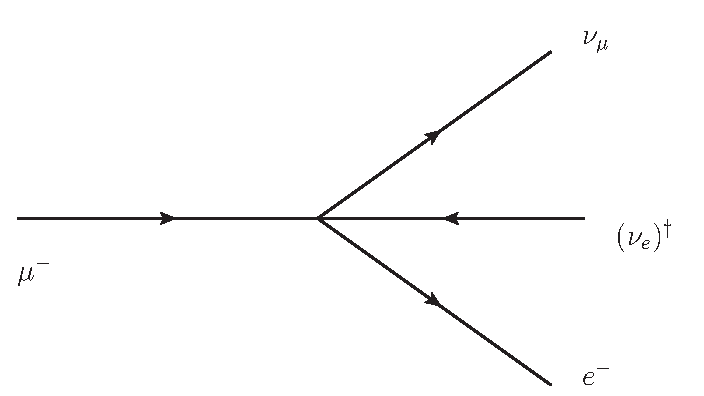
\includegraphics[scale=0.8]{mucontact}  
  \caption{Decaimiento del muón a tres cuerpos}
  \label{fig:mucontact}
\end{figure}

Construyendo la misma interacción a partir del Lagrangiano del ME
\begin{align}
  \mathcal{L}=&\frac{g_2^2}{8}\left[\bar{\nu}_\mu\gamma^\mu(1-\gamma_5)\mu\right] \left[ W_{\mu}^{+}W_\nu^{-} \right]
  \left[\bar{e}\gamma^\nu(1-\gamma_5)\nu_e\right]\,.
\end{align}
Por lo tanto la contracción apropiada de $\left[ W_{\mu}^{+}W_{\nu}^{-} \right]$ debe generar el coeficiente inverso de masa al cuadrado:
\begin{align}
  \left[ W_{\mu}^{+}W_\nu^{-} \right]\to \frac{1}{m_W^2}\,.
\end{align}
Una deducción más rigurosa se realizará en la Sección~\ref{sec:deca-debil-medi}. Por lo tanto
\begin{align}
    \frac{G_F}{\sqrt{2}}=&\frac{g^2}{8m_W^2}\nonumber\\
=& \frac{e^2}{8m_W^2\sin^2\theta_W} \nonumber\\
=& \frac{4\pi e^2}{8(4 \pi) m_W^2\sin^2\theta_W} \nonumber\\
=& \frac{\pi\alpha }{2 m_W^2\sin^2\theta_W} \nonumber\\
m_{W}^2\sin^2\theta_W=&\frac{\sqrt{2}\pi\alpha }{2 G_F} \nonumber\\
m_{W}^2\sin^2\theta_W=&\frac{\pi\alpha }{\sqrt{2} G_F} \,.
\end{align}

Además, de la ec.~\eqref{eq:mwzw}
\begin{align}
  \cos^2\theta_W=&\frac{m_W^2}{m_Z^2} \nonumber\\
  1-\sin^2\theta_W=&\frac{m_W^2}{m_Z^2} \nonumber\\
  \sin^2\theta_W=&1-\frac{m_W^2}{m_Z^2} \,.
\end{align}


De esta forma tenemos las relaciones
\begin{align}
  \sin^2\theta_W=&1-\frac{m_W^2}{m_Z^2}\,,&m_W^2\sin^2\theta_W=\frac{\pi\alpha}{\sqrt{2}G_F}\,,
\end{align}
que permiten determinar que
\begin{align}
  \sin^2\theta_W\approx &0.21\nonumber\\
  m_W\approx &81\,\text{GeV}\,.
\end{align}
El uso de $\alpha(M_Z)\approx1/128$, permite tener en cuenta algunas correcciones cuánticas dando lugar a
\begin{align}
   \sin^2\theta_W\approx &0.23\nonumber\\
  m_W\approx &80\,\text{GeV}
\end{align}
Los valores medidos son $\sin^2\theta_W=0.23149(13)$, $m_W=80.398(25)\,$GeV, y pueden ser reproducidos por el modelo estándar una vez se tienen en cuenta correcciones perturbativas inducidas por partículas virtuales.

El acelerador $e^+e^-$ LEP, que funcionó desde 1998 hasta el 2000~\cite{LEP}, operó a energías suficientes para producir millones de $Z$. Combinado con otros resultados experimentales, se pudo verificar todo el Lagrangiano del Modelo Estándar hasta un nivel del 1 por mil. Con excepción de las interacciones asociadas con el Higgs. 

La universalidad de los decaimientos del $Z$ está soportada por los resultados experimentales siguientes donde sólo se muestran los decaimientos leptónicos del $Z$ diferentes de cero \cite{a} 
\begin{align}
  \label{eq:232qft}
  \Gamma(Z\to e^+e^-)&=83.92(12)\,\text{MeV} &\Gamma(Z\to\mu^+\mu^-)&=83.99(18)\,\text{MeV} 
  &\Gamma(Z\to\tau^+\tau^-)&=84.08(22)\,\text{MeV} \nonumber\\
  \operatorname{Br}(Z\to e^+e^-)&=3.363(4)\%, &\operatorname{Br}(Z\to\mu^+\mu^-)&=3.366(7)\%,  &
  \operatorname{Br}(Z\to\tau^+\tau^-)&=3.370(8)\% 
\end{align}
Mientras que para el $W^\pm$, en \%, \cite{pdg}
\begin{align}
\label{eq:231qft}
  \operatorname{Br}(W^-\to\bar{\nu}_e e^-)&=10.71(16), &
\operatorname{Br}(W^-\to\bar{\nu}_\mu \mu^-)&=10.63(15), &
\operatorname{Br}(W^-\to\bar{\nu}_\tau \tau^-)&=11.38(21)\,. 
\end{align}
La diferencia de $\bar{\nu}_\tau \tau$ respecto a los otros representa un efecto alrededor de $2\sigma$. La universalidad de los acoplamientos leptónicos de $W$ puede comprobarse también indirectamente a través de los decaimientos débiles mediados por corrientes cargadas. Los datos actuales verifican la universalidad de los acoplamientos de corrientes cargadas leptónicas al nivel del 0.2\%~\cite{a}. Sin necesidad de entrar en detalles de los cálculos de las amplitudes de decaimiento, podemos usar el hecho de que ellas son proporcionales a los acoplamientos al cuadrado correspondiente, de modo que  un cociente entre amplitudes de decaimiento es igual, en primera aproximación, a los cocientes de los acoplamientos al cuadrado. Tendremos en cuenta además que el Branching es la amplitud de decaimiento a un canal especifico divido por la suma de las amplitudes de decaimiento a todos los canales posibles.




Para los decaimientos del $Z$ el Modelo Estándar predice, además de la ausencia de eventos del tipo $Z\to e^+\mu^-$, que para un cierto  $l=e,\mu,\tau$, o  $q=d,s,b$
\begin{align}
  \frac{ \operatorname{Br}(Z\to l^+l^-)}{ \operatorname{Br}(Z\to\bar{q}q)}\approx&
\frac{(|v_l|^2+|a_l|^2)}{N_c(|v_q|^2+|a_q|^2)}\nonumber\\
=&\frac{\left[\left(-\frac{1}{2}+2\sin^2\theta_W\right)^2+\frac{1}{4}\right]}{
N_c\left[\left(-\frac{1}{2}+\frac{2}{3}\sin^2\theta_W\right)^2+\frac{1}{4}\right]}\nonumber\\
\approx&\frac{0.776}{N_c}=
\begin{cases}
  0.338& N_c=2\\
  0.225& N_c=3\\
  0.169& N_c=4
\end{cases}
\end{align}
Para ser comparado con el resultado experimental de por ejemplo
\begin{align}
  \frac{ \operatorname{Br}(Z\to e^+e^-)}{ \operatorname{Br}(Z\to\bar{b}b)}=\frac{3.363(4)}{15.12(5)}\approx0.222
\end{align}
que de nuevo da lugar al $N_c=3$, que seguiremos tomando en adelante.

Los Branchings de decaimiento en la ec.~\eqref{eq:231qft} y ec.~\eqref{eq:232qft}  pueden ser calculados sin entrar en detalles del cálculo de las amplitudes. Teniendo en cuenta que el canal $Z\to\bar{t}t$ esta cerrado
\begin{align}
  &\operatorname{Br}(Z\to e^+e^-)=\frac{\Gamma(Z\to e^+e^-)}{\Gamma_{\text{total}}}\nonumber\\
 &\qquad=\frac{(|v_e|^2+|a_e|^2)}{\sum_l[(|v_l|^2+|a_l|^2)+(|v_{\nu_l}|^2+|a_{\nu_l}|^2)]
+N_c[\sum_{i=1}^2(|v_{u_i}|^2+|a_{u_i}|^2)+\sum_{i=1}^3(|v_{d_i}|^2+|a_{d_i}|^2)]}\nonumber\\
 &\qquad=\frac{(|v_e|^2+|a_e|^2)}{3[(|v_e|^2+|a_e|^2)+(|v_{\nu_e}|^2+|a_{\nu_e}|^2)]
+3[2(|v_{u}|^2+|a_{u}|^2)+3(|v_{d}|^2+|a_{d}|^2)]}\nonumber\\
  &\qquad=\frac{(|v_e|^2+|a_e|^2)}{21|a_e|^2+3[|v_e|^2+|v_{\nu_e}|^2]
+3[2|v_{u}|^2+3|v_{d}|^2]}\nonumber\\
 &\qquad=\frac{(-1+4s^2\theta_W)^2+1}{21+3[(-1+4s^2\theta_W)^2+1]
+3[2(1-\frac{8}{3}s^2\theta_W)^2+3(-1+\frac{4}{3}s^2\theta_W)^2]}\nonumber\\
  &\qquad=\frac{2-8s^2\theta_W+16s^4\theta_W}{42-80s^2\theta_W+\frac{320}{3}s^4\theta_W}\nonumber\\
&\qquad\approx3.43\%
\end{align}
Para $W^\pm$ tenemos por ejemplo
\begin{align}
\operatorname{Br}(W^-\to\bar{\nu}_e e^-)=\frac{\Gamma(W^-\to\bar{\nu}_e e^-)}{\Gamma_{\text{total}}}
\end{align}
donde, teniendo en cuenta que los canales a top están cerrados, y usando la condición de unitariedad de la matriz CKM en ec.~\eqref{eq:230qft}, tenemos
\begin{align}
  \Gamma_{\text{total}}=&\sum_l\Gamma(W^-\to\bar{\nu}_l l^-)+N_c\sum_i[\Gamma(W^-\to\bar{u}_1d_i)+\Gamma(W^-\to\bar{u}_2d_i)]\nonumber\\
  =&\Gamma(W^-\to\bar{\nu}_e e^-)\{3+N_c\sum_i[|V_{1i}|^2+|V_{1i}|^2]\} \nonumber\\
  =&\Gamma(W^-\to\bar{\nu}_e e^-)(3+2N_c) \nonumber\\
\end{align}
entonces
\begin{align}
  \operatorname{Br}(W^-\to\bar{\nu}_e e^-)=\frac{1}{3+2N_c}=11.1\%
\end{align}
Una mejor predicción de dichos resultados en el contexto del Modelo Estándar requiere tener en cuenta las correcciones radiativas.


El ME también tiene una predicción concreta para la amplitud del $Z$ a neutrinos, $\Gamma_{\text{inv}}$:
\begin{align}
  \frac{\Gamma_{\text{inv}}}{\Gamma_l}=&\frac{\sum_l\Gamma(Z\to\bar{\nu}_l\nu_l)}{\Gamma(Z\to e^+ e^-)}\nonumber\\
  &=\frac{N_\nu\Gamma(Z\to\bar{\nu}_e\nu_e)}{\Gamma(Z\to e^+ e^-)}\nonumber\\
  &\approx\frac{N_\nu(|v_{\nu_e}|^2+|a_{\nu_e}|^2)}{|v_{e}|^2+|a_{e}|^2}\nonumber\\
  &=\frac{2N_\nu}{(-1+4\sin^2\theta_W)^2+1}\nonumber\\
  &=\frac{N_\nu}{1-4\sin^2\theta_W+8 \sin^4\theta_W}\nonumber\\
  &\approx\begin{cases}
    5.865&N_\nu=3\\
    7.819&N_\nu=4
  \end{cases}\,,
\end{align}
mientras que el valor medido experimentalmente para esta cantidad $5.942(16)$ \cite{a}, es una evidencia muy fuerte de que sólo exiten tres neutrinos livianos. 
\end{frame}

Note que el mismo resultado se puede obtener usuando la notación de dos componentes de \eqref{eq:lsmw}. Con $t_{e_R}=0$, $t_{\nu}=-t_{e_L}=1$, $Q_{\nu}=0$ y $Q_e=-1$ tenemos que
\begin{align}
  \frac{\Gamma_{\text{inv}}}{\Gamma_l}=&\frac{\sum_l\Gamma \left[ Z\to \left( \nu_l \right)^{\dagger}\nu_l \right]}{\Gamma \left[Z\to \left( e_L \right)^{\dagger} e_L  \right]+\Gamma \left[Z\to \left( e_R \right)^{\dagger} e_R  \right]}\nonumber\\
=&\frac{N_{\nu} t_{\nu}^2 }{\left( t_{e_L} - 2 Q_e \sin^2\theta_W \right)^2+ \left( 2 Q_e \sin^2\theta_W \right)^2 } \nonumber\\
=&\frac{N_{\nu} }{\left( -1 + 2 \sin^2\theta_W \right)^2+4 \sin^4\theta_W } \nonumber\\
=&\frac{N_{\nu} }{1 - 4 \sin^2\theta_W +4 \sin^4\theta_W +4 \sin^4\theta_W } \nonumber\\
=&\frac{N_{\nu} }{1 - 4 \sin^2\theta_W +8 \sin^4\theta_W } \,.
\end{align}

\subsection{Decaimientos débiles mediados por corrientes cargadas}
\label{sec:deca-debil-medi}
\begin{frame}[fragile,allowframebreaks]
De la corrientes cargadas para leptones tenemos
\begin{align}
  \mathcal{L}_{cc}\supset&\frac{g_2}{2\sqrt{2}}\left[\sum_l\bar{\nu_l}\gamma^\mu(1-\gamma_5)l W_\mu^++\bar{l}\gamma^\mu(1-\gamma_5)\nu_l W_\mu^-\right]
\end{align}
Esto da lugar a los posibles diagramas para decaimientos de leptones a bosones virtuales, y bosones a leptontes mostrados en la figura~\ref{fig:leptoncc}. Las flechas representan el flujo de número leptónico. La flecha de tiempo es de izquierda a derecha. Al lado izquierdo del vértice entran partículas y salen antipartículas. Mientras que al lado derecho entran antip artículas y salen partículas
\begin{figure}
  \centering
  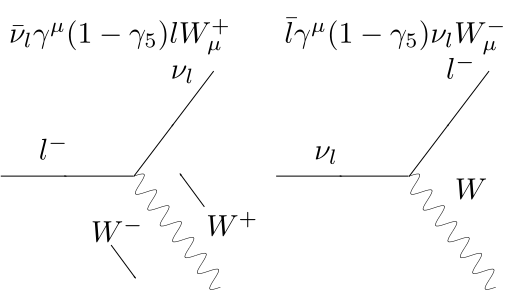
\includegraphics[scale=0.5]{leptoncc}
\qquad  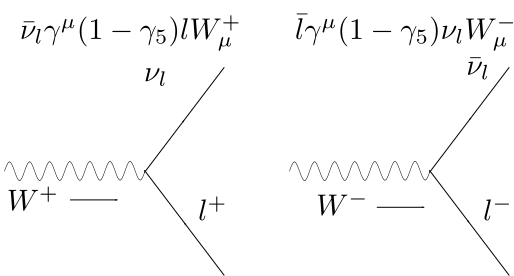
\includegraphics[scale=0.5]{wdecay}

  \caption{Diagramas de Feynman para las corrientes cargadas}
  \label{fig:leptoncc}
\end{figure}
Del primer y cuarto diagrama obtenemos el diagrama de Feynman para el decaimiento $\mu^-\to \nu_\mu e^-\bar{\nu}_e$, mostrado en la figura~\ref{fig:muondecay}
\begin{figure}
  \centering
  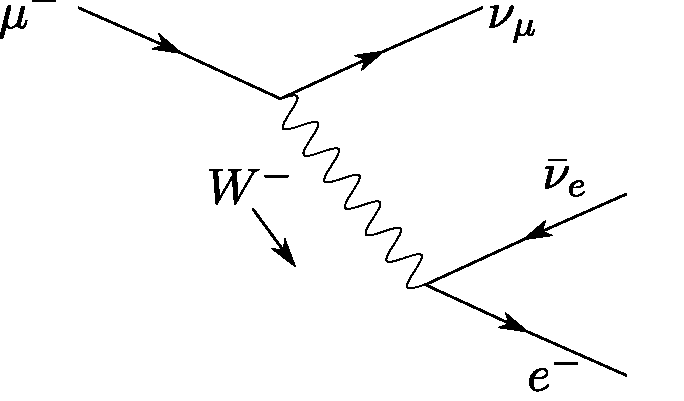
\includegraphics[scale=0.5]{muon_decay}
  \caption{diagrama de Feynman para el decaimiento $\mu^-\to \nu_\mu e^-\bar{\nu}_e$}
  \label{fig:muondecay}
\end{figure}
El propagador para el bosón $W$ de momentum $q$ resulta ser
\begin{align}
  \widetilde{D}_{\mu\nu}=\frac{1}{q^2-m_W^2}\left(g_{\mu\nu}-\frac{q_\mu q_\nu}{m_W^2}\right)\,.
\end{align}
Para los propósitos actuales la obtención de este resultado no es necesaria, el punto importante es que cuando los momentum de las partículas iniciales y finales son mucho más pequeñas que $m_W$, esto se reduce a
\begin{align}
  \widetilde{D}_{\mu\nu}=-\frac{g_{\mu\nu}}{m_W^2}\,.
\end{align}
Este resultado se entiende fácilmente cuando se compara con el propagador de una partículas escalar masiva $1/(q^2-M^2)\to-1/M^2$. Las componentes espaciales de $W_\mu$ con $\mu=1,2,3$, a bajas energías tienen el mismo propagador que el de una partícula escalar, mientras $W_0$, tiene el signo opuesto.

El Lagrangiano efectivo para el decaimiento del muón, $\mu^-\to \nu_\mu e^- \bar{\nu}_e$ es entonces
\begin{align}
  \mathcal{L}=&\frac{g_2^2}{8}\left[\bar{\nu}_\mu\gamma^\mu(1-\gamma_5)\mu\right]\frac{g_{\mu\nu}}{m_W^2}
  \left[\bar{e}\gamma^\nu(1-\gamma_5)\nu_e\right]\nonumber\\
=&\frac{g_2^2}{8m_W^2}\left[\bar{\nu}_\mu\gamma^\mu(1-\gamma_5)\mu\right]
  \left[\bar{e}\gamma^\nu(1-\gamma_5)\nu_e\right]\nonumber\\
  =&\frac{G_F}{\sqrt{2}}\left[\bar{\nu}_\mu\gamma^\mu(1-\gamma_5)\mu\right]\left[\bar{e}\gamma_\mu(1-\gamma_5)\nu_e\right]\,,
\end{align}
donde
\begin{align}
  \frac{G_F}{\sqrt{2}}=&\frac{g_2^2}{8m_W^2}\nonumber\\
  =&\frac{g_2^24}{8g^2v^2}\nonumber\\
  =&\frac{1}{2v^2}\,,
\end{align}
y
\begin{align}
  v=\left(\sqrt{2}\,G_F\right)^{-1/2}=&246.2\ \text{GeV}\nonumber\\
 \approx&2.9\times 10^{15}\ \text{K} \nonumber\\
 \approx&4.9\times 10^{-14}\ \text{m} \nonumber\\
 \approx&1.6\times 10^{-22}\ \text{s} \,.
\end{align}


De otro lado, para el  decaimiento $\beta$, $n\to p e^- \bar{\nu}_e$, de acuerdo a la figura~\ref{fig:neutrondecay}, tenemos

\begin{align}
    \mathcal{L}=\frac{G_\beta}{\sqrt{2}}\left[\bar{p}\gamma^\mu(1-1.26\gamma_5)n\right]\left[\bar{e}\gamma_\mu(1-\gamma_5)\nu_e\right]\,.
\end{align}
\begin{figure}
  \centering
  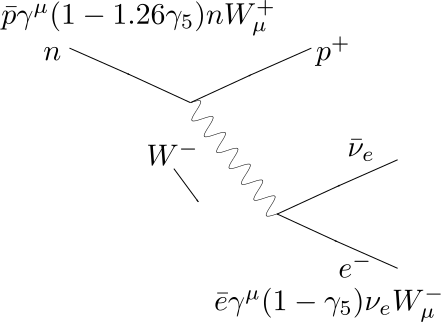
\includegraphics[scale=0.5]{neutrondecay}
  \caption{Decaimiento del neutrón.}
  \label{fig:neutrondecay}
\end{figure}
con $G_F$ dado en la ec.~\eqref{eq:233qft} y $G_\beta=1.10\times 10^{-5}\,\text{GeV}^2$. La corriente hadrónica tiene la forma V--1.26A. El factor 1.26  puede entenderse como debido a las correcciones a nivel hadrónico de una corriente que es de la forma V--A a nivel del quarks, como en la ec.~\eqref{eq:234qft}. A nivel de quarks el decaimiento del neutrón ($udd$) al protón ($uud$) corresponde al decaimiento de uno de los quarks down del neutrón $d\to u e^- \bar{\nu}_e$
\begin{align}
    \mathcal{L}=\frac{G_F}{\sqrt{2}}V_{11}\left[\bar{u}\gamma^\mu(1-\gamma_5)d\right]\left[\bar{e}\gamma_\mu(1-\gamma_5)\nu_e\right]\,.
\end{align}
De modo que $G_\beta=G_F V_{11}=G_F\cos\theta_C$, donde $\theta_C$ es el ángulo de Cabbibo. Una vez se tienen en cuenta correcciones electrodébiles se obtiene el valor $|V_{11}|=0.97418(27)$\cite{PDG}. Las magnitudes de los elementos de la matriz CKM son\cite{PDG}
\begin{align}
  V\approx\begin{pmatrix}
    0.97419&0.2257&0.0359\\
    0.2256&0.97334&0.0415\\
    0.00874&0.0407&0.999133
  \end{pmatrix}\sim \mathbf{1}
\end{align}
\end{frame}

Para cerrar esta notas, transcribo a continuación el último párrafo de la conferencia de Steven Weinberg en 1979 con motivo de la entrega del premio nobel del física por el desarrollo del modelo estándar de las interacciones fundamentales:

\begin{quote}
[...]  And
nothing makes me more optimistic than the discovery of broken symmetries.
In the seventh book of the Republic, Plato describes prisoners who are
chained in a cave and can see only shadows that things outside cast on the
cave wall. When released from the cave at first their eyes hurt, and for a
while they think that the shadows they saw in the cave are more real than
the objects they now see. But eventually their vision clears, and they can
understand how beautiful the real world is. We are in such a cave, imprisoned
by the limitations on the sorts of experiments we can do. In particular,
we can study matter only at relatively low temperatures, where symmetries
are likely to be spontaneously broken, so that nature does not appear
very simple or unified. We have not been able to get out of this cave, but by
looking long and hard at the shadows on the cave wall, we can at least make
out the shapes of symmetries, which though broken, are exact principles
governing all phenomena, expressions of the beauty of the world outside.
\end{quote}
S. Weinberg, Nobel lecture, 1979

\section{Resumen}
A modo de resumén, usaremos a continuación la siguiente secuencia de la historieta de \url{http://www.phdcomics.com} re-explicando el bosón de Higgs:
\newpage

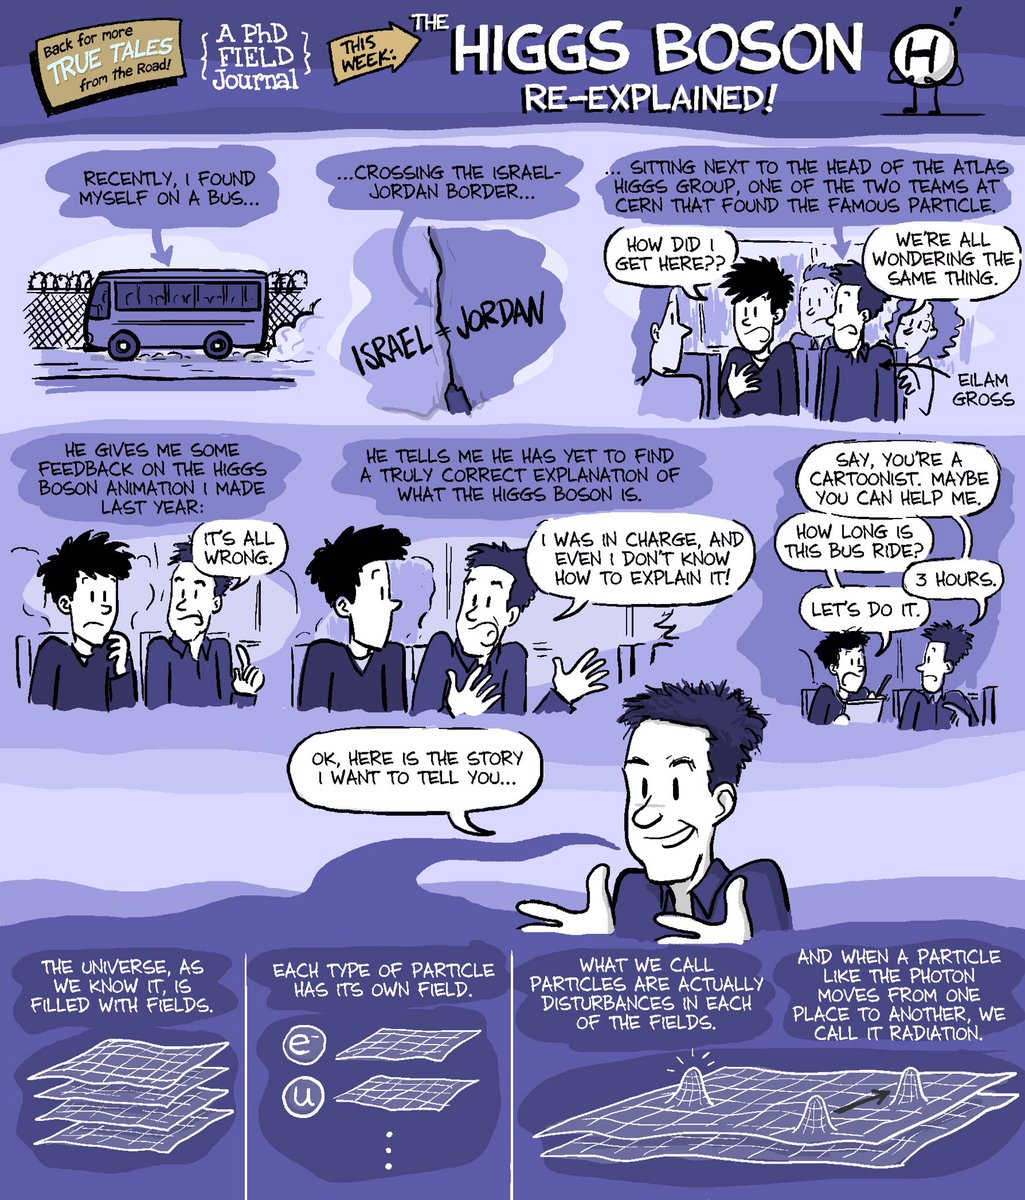
\includegraphics[scale=0.51]{Higgs1}

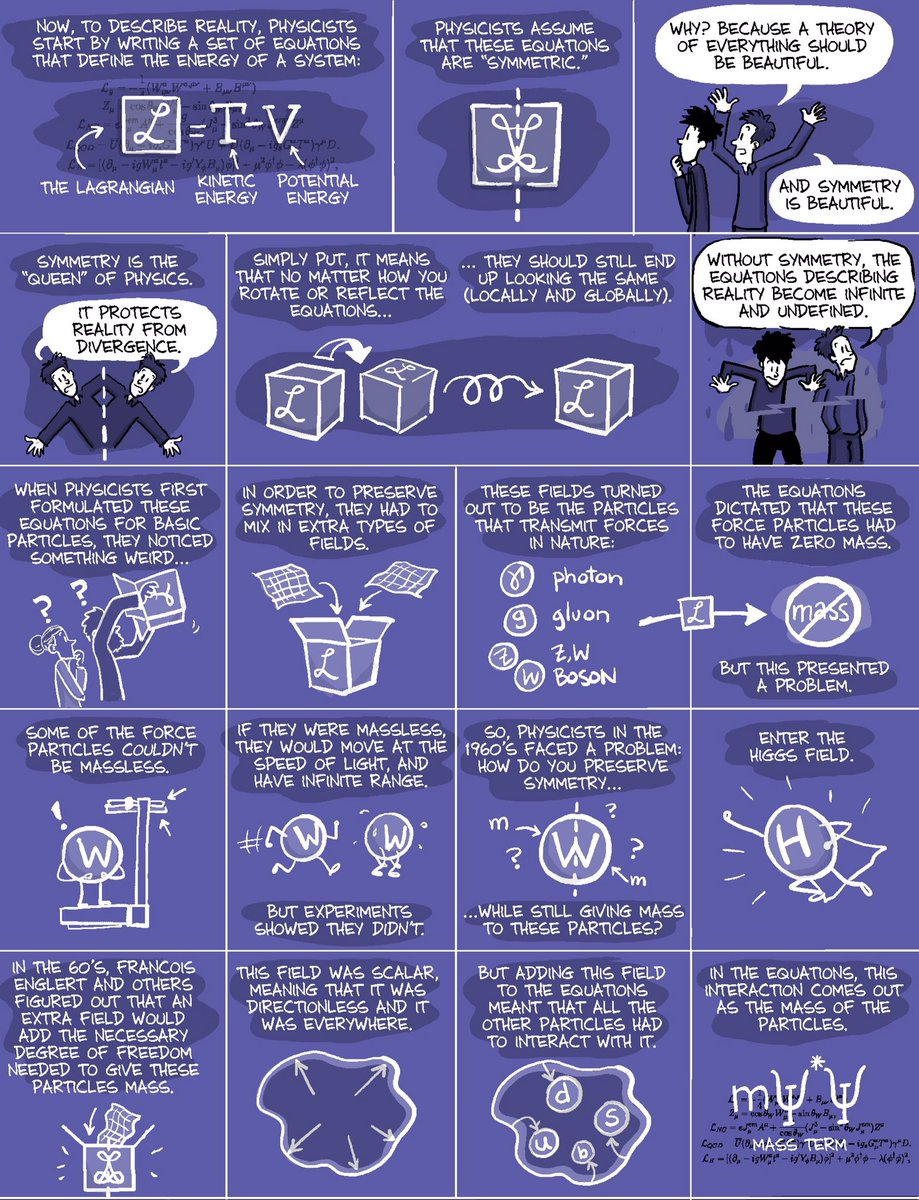
\includegraphics[scale=0.56]{Higgs2}

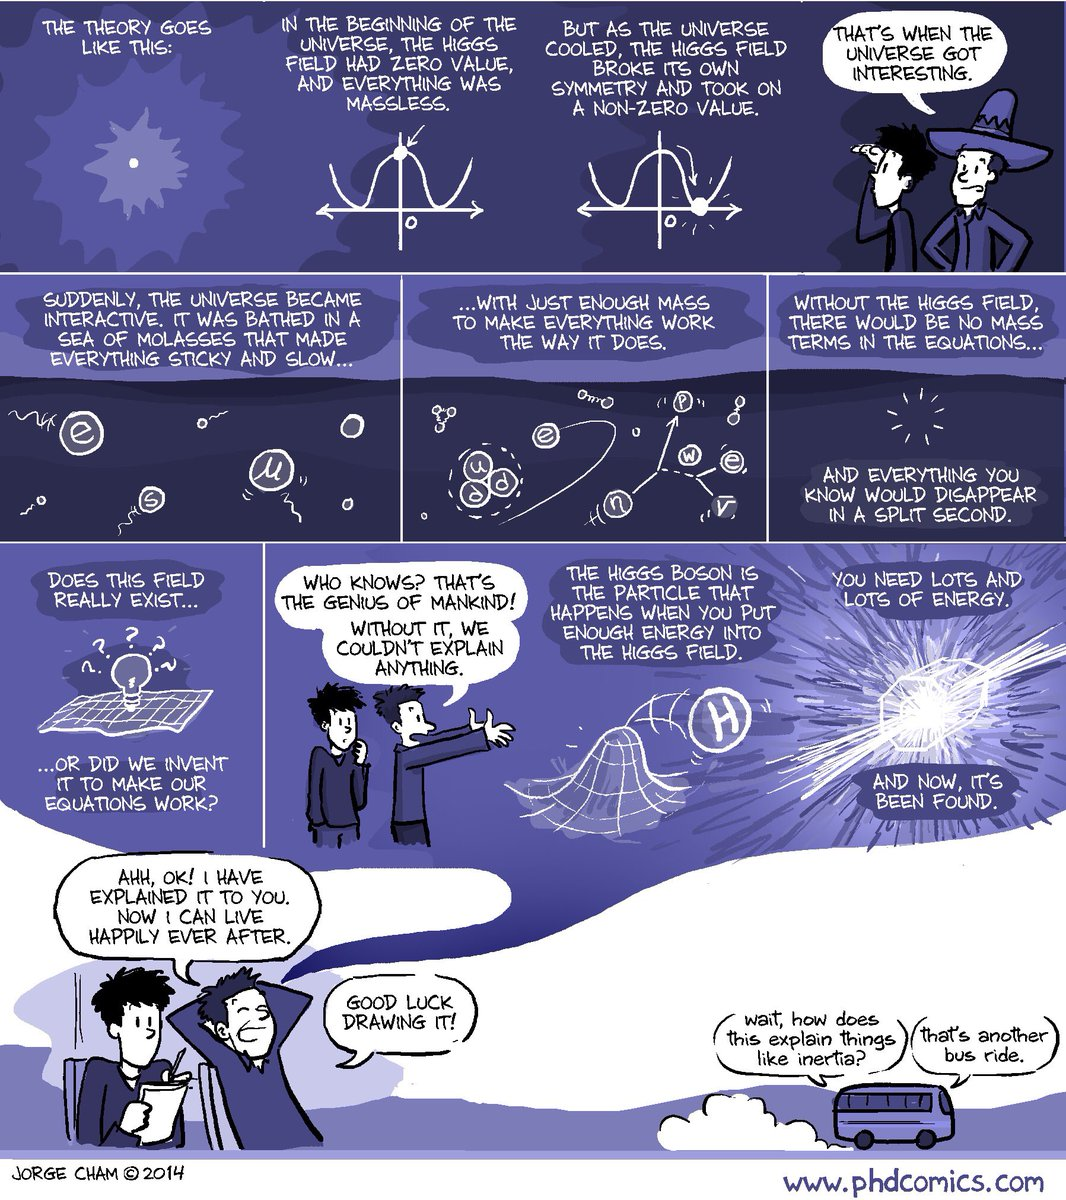
\includegraphics[scale=0.49]{Higgs3}

\newpage


\section{Lecturas recomendadas}
Libros:
\begin{itemize}
\item \cite{kane,cottingham,Pich:2005mk}
\end{itemize}

Artículos originales

\begin{itemize}
\item Teorías no abelianas \cite{Yang:1954ek}
\item Mecanismo de Higgs \cite{Higgs:1964pj}
\item Teoría electrodébil \cite{Weinberg:1967tq}
\end{itemize}

Artículo de divulgación
\begin{itemize}
\item The deconstructed Standard Model equation, Rashmi Shivni \url{https://www.symmetrymagazine.org/article/the-deconstructed-standard-model-equation}
\end{itemize}

Videos:
\begin{itemize}
\item Strange Stars Explained: \url{https://www.youtube.com/watch?v=p_8yK2kmxoo}
\end{itemize}

% \left(\right)
%
%%% Local Variables: 
%%% mode: latex
%%% TeX-master: "fullnotes"
%%% ispell-local-dictionary: "castellano8"
%%% End:
